\documentclass[12pt, a4paper, oneside]{ctexbook}
\usepackage{amsmath, amsthm, amssymb, bm, graphicx, hyperref, mathrsfs}
\usepackage{geometry}
\usepackage{float}
\geometry{a4paper, left=2.5cm, right=2.5cm, top=2.5cm, bottom=2.5cm}
\usepackage{titlesec}
\titleformat{\chapter}[display]
  {\Huge\bfseries}
  {\chaptername\ \thechapter}
  {0pt}
  {\Huge}

\titleformat{\section}
  {\Large\bfseries}
  {\thesection}
  {1em}
  {}

\titleformat{\subsection}
  {\large\bfseries}
  {\thesubsection}
  {1em}
  {}

\title{{\Huge{\textbf{Probability Distribution}}}\\}
\author{梁云森}
\date{\today}
\linespread{1.5}
\newtheorem{theorem}{定理}[section]
\newtheorem{definition}[theorem]{定义}
\newtheorem{lemma}[theorem]{引理}
\newtheorem{corollary}[theorem]{推论}
\newtheorem{example}[theorem]{例}
\newtheorem{proposition}[theorem]{命题}

\begin{document}

\maketitle

\pagenumbering{roman}
\setcounter{page}{1}

\begin{figure}[H]
  \centering
  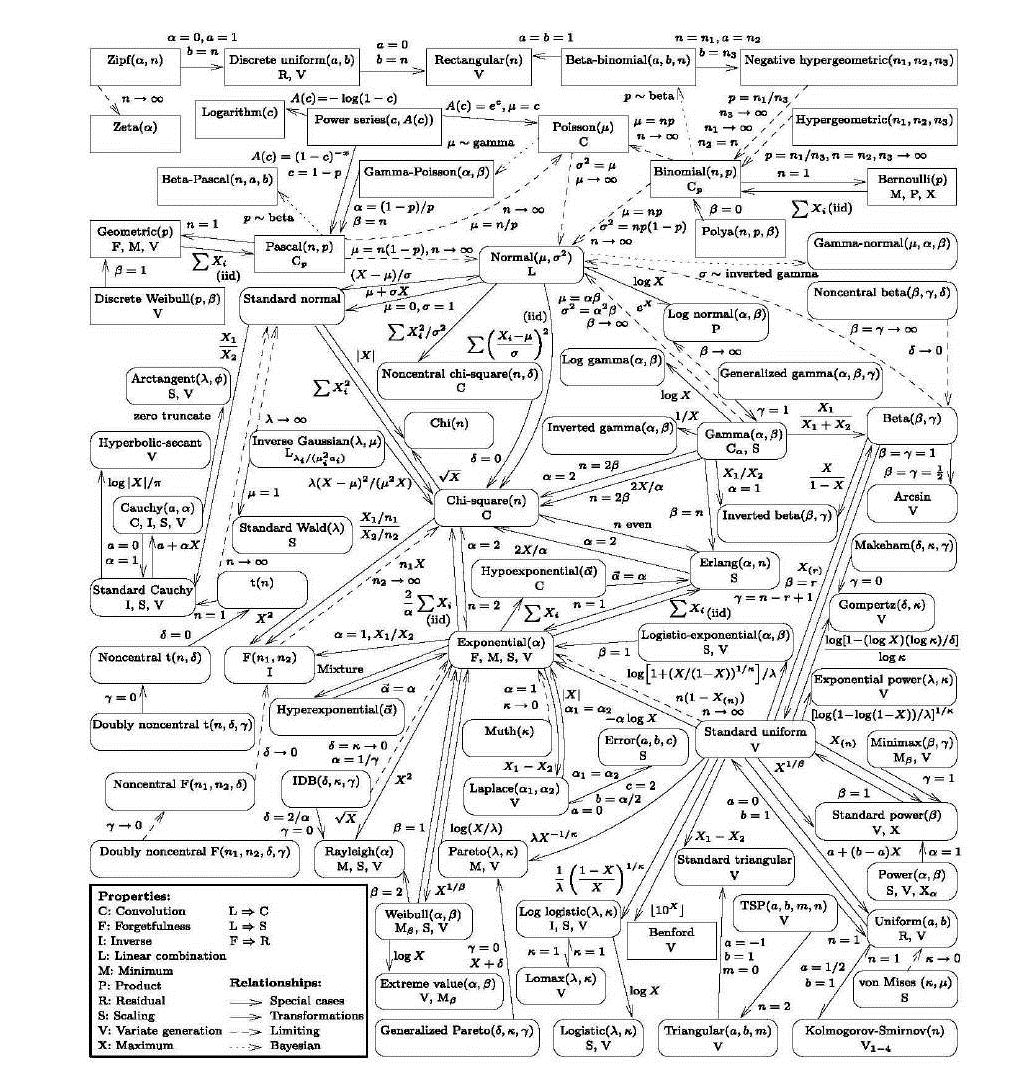
\includegraphics[width=1\textwidth]{image/分布大全.png}
  \label{fig:example}
\end{figure}

\textbf{\Large{Wir müssen wissen. Wir werden wissen.t}}
~\\
\begin{flushright}
    \begin{tabular}{c}
        David Hilbert
    \end{tabular}
\end{flushright}

\newpage
\pagenumbering{Roman}
\setcounter{page}{1}
\tableofcontents
\newpage
\setcounter{page}{1}
\pagenumbering{arabic}

\chapter{离散分布}

\section{Bernoulli 分布(Bernoulli Distribution)}

符号:$X \sim B(1, p)$

概率:$P(X = k) = p^{k}(1-p)^{1-k}$

期望:$E(X) = 0\times (1-p) + 1 \times p = p$ 

方差:$D(X) = E(X^{2}) - E(X)^{2} = p - p^2 = p(1-p)$

应用:

1. 伯努利分布常常用于描述二元随机试验的结果,如硬币投掷(正面或反面)、赌博游戏中的赢或输、产品的合格或不合格等。

2. 伯努利分布是二项分布(Binomial Distribution)的特例,当进行多次独立的伯努利试验时,可以通过多次伯努利试验的求和得到二项分布。

3. 在机器学习中,伯努利分布常用于建模二元分类问题,其中一个例子是垃圾邮件过滤,其中每封电子邮件被视为一个伯努利试验,成功表示是垃圾邮件,失败表示不是。

\section{二项分布(Binomial Distribution)}

 符号:$X\sim B(n, p)$
 
 概率:
$$
P(X = k) = \begin{pmatrix}
n \\
k
\end{pmatrix} (1-p)^{n - k}p^k
$$

期望:

\begin{align*}
    E(X)= \sum\limits_{k = 0}^{n}kp(X = k) =\sum\limits_{k = 0}^{n} k\begin{pmatrix}
n \\
k
\end{pmatrix} (1-p)^{n - k}p^k \\
= \sum\limits_{k = 1}^{n}\begin{pmatrix} n - 1\\ m - 1\end{pmatrix}p^{k}(1-p)^{n - k} \quad \quad \quad \\
= \sum\limits_{k = 0}^{n - 1}np\begin{pmatrix}n - 1 \\ k \end{pmatrix} p^{k}(1-p)^{n - 1 - k} \quad \\
= np\times (p + (1 - p))^{n - 1} \quad \quad \quad \quad \quad  \\
= np \quad \quad \quad \quad \quad \quad \quad \quad \quad \quad \quad \quad \quad
\end{align*}

 方差:

\begin{align*}
D(X) = E(X^{2}) - E(X)^{2} =E(X(X-1)+X) - E(X)^{2} \\
=E(X(X-1)) + E(X) - E(X)^{2} \quad \quad \quad \quad  \\
\end{align*}
\begin{align*}
    E(X(X-1)) &= \sum\limits_{k = 0}^{n}k(k - 1)\begin{pmatrix} n \\ k\end{pmatrix} p^{k}(1-p)^{n - k}  \\ &= n(n - 1)\sum\limits_{k = 2}^{n} \begin{pmatrix} n - 2\\ k - 2\end{pmatrix} p^{k}(1 - p)^{n - l}  \\
&= n(n - 1)\sum\limits_{k = 0}^{n - 2}\begin{pmatrix} n - 2 \\ k \end{pmatrix} p^{k + 2}(1-p)^{n - 2 - k} \\
&= n(n - 1) p^{2} (1 + (1 - p))^{n - 2}  \\
&= n(n - 1)p^{2} \\
\end{align*}
\begin{align*}
    D(X) = n(n -1)p^{2} + np - n^{2}p^{2}  = np(1-p) 
\end{align*}


 性质:
 
二项分布与泊松分布之间的关系:当二项分布的试验次数 n 很大,成功概率 p 很小,使得平均发生率 λ = np 保持不变时,二项分布可以近似为泊松分布。这是因为在这种情况下,二项分布中的事件之间的间隔趋向于变得很小,类似于泊松分布中的随机事件计数。

 应用:
 
1. 一段时间内物理实验仪器捕获的粒子数目。

2. 一段时间内计算机病毒的入侵数。

3. 一本书中的错字数。

\section{多项分布(Multinomial Distribution)}

多项分布(Multinomial Distribution),它是二项分布的推广。二项分布的试验结果只有两个(成功和失败),而多项分布的试验结果则多于两个。

联合概率函数:

\begin{align*}
    P(X_1 = x_1, X_2 = x_2, ..., X_k = x_k) = \dfrac{n!}{x_1!x_2!...x_k!} p_1^{x_1}p_2^{x_2}...p_{k}^{x_k}
\end{align*}

多项分布对于每一个结果都有均值和方差,分别为:

 期望:
$$
E(X_i) = np_i
$$

 方差:

$$
D(X_i) = np_i(1-p_i)
$$


\section{泊松分布(Possion Distribution)}

符号:$X\sim P(\lambda)$

概率:$P(X = x) = \dfrac{e^{-\lambda}\lambda^{x}}{x!}$

证明:

由 $\lambda$ 的定义,单位时间内随机事件发生 $\lambda$ 次,并且每一次事件发生都是独立的,和时间没有关系的。
所以如果我们将单位单位时间划分为 n 份,当 n 趋近于正无穷的时候,我们可以认为每一段时间内事件发生的次数是均匀的。所以每一段时间事件发生的概率都是 $\dfrac{\lambda}{n}$
$$
P(X = x) = \lim\limits_{n \to +\infty}\begin{pmatrix} n \\ x\end{pmatrix} (\dfrac{\lambda}{n})^{x}(1 - \dfrac{\lambda}{n})^{n - x} = \dfrac{\lambda^{k}}{k!}e^{-\lambda}
$$

期望:

$$
\begin{aligned}
E(X) &= \sum\limits_{k=0}^{+\infty} k \dfrac{\lambda^{k}}{k!}e^{-\lambda} \\
&= \lambda e^{-\lambda} \sum\limits_{k = 1}^{+\infty} \dfrac{\lambda^{k - 1}}{(k - 1)!} \\
&= \lambda e^{-\lambda} e^{\lambda} \\
&= \lambda
\end{aligned}
$$

方差:

\begin{align*}
E(X^{2}) &= E(X(X - 1) + X) = E(X(X-1)) + E(X) \\
E(X(X - 1)) &= \sum\limits_{k = 1}^{+\infty} k(k - 1) \dfrac{\lambda^{k}}{k!}e^{-\lambda} \\&=\sum\limits_{k = 2}^{+\infty}\dfrac{\lambda^{k}}{(k - 2)!}e^{-\lambda} \\
&= \lambda^{2}e^{-\lambda}\sum\limits_{k = 0}^{+\infty}\dfrac{\lambda^{k}}{k!}\\&= \lambda^{2}\\D(X) &= E(X^{2}) - E(X)^{2} \\&= E(X(X - 1)) + E(X) - E(X)^{2} \\&= \lambda^{2} + \lambda - \lambda^{2}\\&= \lambda
\end{align*}

性质:

1. 伯努利分布是二项分布的特殊情况,当 n = 1 的时候,二项分布变为伯努利分布。泊松分布可以被看作是二项分布的极端情况,在试验次数非常多或者成功概率非常小的情况下,可以近似为泊松分布。指数分布也可以由泊松分布推导而来。

2. 泊松分布中 $\lambda$ 表示单位时间内随机事件的平均发生次数。在一个特定时间内,某一个事件都会在任意时刻发生(前提是,每次发生都是独立的,并且跟事件没有关系)。

应用:

泊松分布是用来描述在给定时间段内随机事件发生次数的分布。

1. 自然科学:泊松分布常用于描述自然界中随机事件的发生,如地震的频率、闪电的击中次数、放射性核素的衰变事件等。

2. 生物学:在生态学和生物学中,泊松分布用于描述生物种群中的种群数量分布、疾病传播的计数、个体的繁殖次数等。

3. 一天之间收到的电子邮件数量。

\section{几何分布(Geometric Distribution)}

 符号:$X\sim G(p)$

 概率:$P(X = k) = (1-p)^{k - 1}p$

所谓「几何分布」,其实就是分布列各项构成等比数列,而等比数列又叫做「几何数列」(源于除了首项和末项意外,每一项都是前后两项的几何平均数)

 期望:

\begin{align*}
E(X) &= \sum\limits_{k = 1}^{+\infty} k \cdot (1-p)^{k - 1}p \\
&=p \sum\limits_{k = 1}^{+\infty} \left( \int k \cdot (1-p)^{k - 1}\right)' \\
&= p \left(-\sum\limits_{k = 1}^{+\infty}(1-p)^{k} \right)' \\
&= p \cdot \dfrac{1}{p^{2}} \\
&= \dfrac{1}{p}
\end{align*}

 方差:


\begin{align*}
D(X) &= E(X^{2}) - E(X)^{2} \\
&= \sum\limits_{k = 1}^{+\infty} k^{2}(1 - p)^{k - 1}p - \dfrac{1}{p^{2}} \\
&= p \left[\sum\limits_{k = 1}^{+\infty}(k+ 1)kq^{k - 1} - \sum\limits_{k = 1}^{+\infty} kq^{k - 1} \right] - \dfrac{1}{p^{2}} \\
&= \dfrac{1 - p}{p^{2}}
\end{align*}


 性质:

1. 离散情况下的「无记忆性」分布,对应连续情况下的「指数分布」。

2. 几何分布通常是右偏的,因为它描述了第一个成功发生所需的试验次数,通常需要等待更长的时间才能获得成功。

\section{超几何分布(Hypergeometric Distribution)}

 符号:$X \sim H(N,n,M)$

 概率:$P(X = k) = \frac{\begin{pmatrix} M \\ k\end{pmatrix} \begin{pmatrix} N - M \\ n - k\end{pmatrix}}{\begin{pmatrix} N \\ M\end{pmatrix}}, k \leq \min(n, M) = k_1$

从上面的「几何分布」我们可以知道,几何二字对应着等比数列。同样的,我们把等比数列的概念推广,数学家们定义了「超几何级数」$\sum\limits_{n = 1}^{+\infty} \beta_n$,它的前一项和后一项之间满足关系 $\dfrac{\beta_{n + 1}}{\beta_n} = \dfrac{P(n)}{Q(n)}$

也就是后一项比前一项是一个 n 的有理函数。

所谓超几何分布,就是分布列的每一项正好是某个超几何级数中的项。

 期望:

$$
\begin{aligned}
E(X) &= \sum\limits_{k = 1}^{k_1} k \cdot \frac{\begin{pmatrix} M \\ k\end{pmatrix} \begin{pmatrix} N - M \\ n - k\end{pmatrix}}{\begin{pmatrix} N \\ M\end{pmatrix}} \\
&= \sum\limits_{k = 1}^{k_1} \begin{pmatrix} N - M \\ n - k\end{pmatrix}\times \frac{\frac{M(M - 1)!}{(k - 1)!(M - k)!}}{\frac{N(N - 1)!}{n(n - 1)!(N-n)!}} \\
&= \dfrac{nM}{N}\sum\limits_{k = 1}^{k_1} \frac{\begin{pmatrix} M - 1 \\ k - 1\end{pmatrix}\begin{pmatrix}N - M \\ n - k \end{pmatrix} }{\begin{pmatrix} N - 1\\ n - 1\end{pmatrix}}\\
&= \dfrac{nM}{N} \frac{\sum\limits_{k = 1}^{k_1} \begin{pmatrix} M - 1 \\ k - 1\end{pmatrix}\begin{pmatrix}N - 1 - (M - 1) \\ n - 1 - (k - 1) \end{pmatrix}}{\begin{pmatrix} N - 1 \\ n - 1\end{pmatrix}} \\
&= \dfrac{nM}{N}
\end{aligned}
$$
 方差:

$$
E(X^{2})= E(X(X - 1) + X) = E(X(X - 1)) + E(X)
$$

$$
\begin{aligned}
E(X(X - 1))) &= \sum\limits_{k = 0}^{k_1} k(k - 1) \frac{\begin{pmatrix}M \\k \end{pmatrix} \begin{pmatrix} N - M \\ n - k\end{pmatrix}}{\begin{pmatrix} N \\ n\end{pmatrix}} \\
&= \frac{nM(n - 1)(M - 1)}{N(N - 1)} \sum\limits_{k = 2}^{k_1} \frac{\begin{pmatrix} M - 2 \\ k - 2\end{pmatrix} \begin{pmatrix} N - M \\ n - k\end{pmatrix}}{\begin{pmatrix} N - 2 \\ n - 2\end{pmatrix}} \\
&= \frac{nM(n - 1)(M - 1)}{N(N - 1)}
\end{aligned}
$$

$$
D(X) = E(X(X - 1))) + E(X) - E(X)^{2}  = \frac{nM(N - M)(N - n)}{N^{2}(N - 1)}
$$

 性质:

1. 当总物品个数远远大于选的个数,或者总物品个数区域无穷大的时候,超几何分布可以近似为二项分布。

 应用:

1. 抽样理论:在质量抽样、生态学调查和生物统计中,超几何分布用于描述非随机抽样情况下的样本中成功的数量,例如从种群中捕捉标记动物的数量。

2. 可靠性工程:在可靠性工程中,超几何分布可用于描述在没有替换的情况下从一个总体中选择样本并确定其中有多少个合格产品。

3. 统计质量控制:超几何分布用于检查生产过程中的样本中不合格产品的数量。

4. 遗传学:在遗传学研究中,超几何分布可用于描述不同基因型的频率分布,以及从种群中选取样本后某一特定基因型的出现次数。

5. 社会科学:在社会调查中,超几何分布可用于描述样本中的各种特征的频率分布,如不同年龄组的人口分布。

\section{负二项分布(帕斯卡分布, Negative Binomial Distribution, Pascal Distribution)}

 符号:$X \sim \text{Pascal}(n, p)$

 概率:$P(X = x) = \begin{pmatrix} x - 1\ \\ r - 1\end{pmatrix}p^{r}(1  -p)^{x - r}$

\begin{figure}[H]
  \centering
  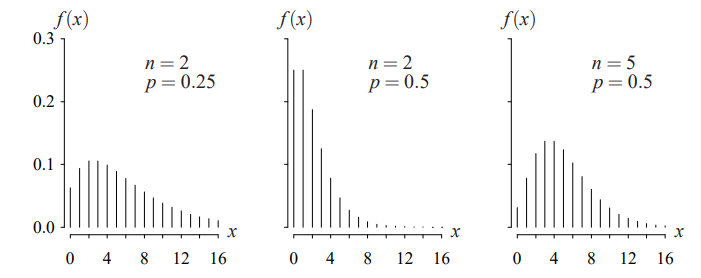
\includegraphics[width=1\textwidth]{image/负二项分布.png}
  \caption{负二项分布}
  \label{fig:example}
\end{figure}

 期望:

$$
\begin{aligned}
E(X) &= \sum\limits_{x = r}^{+\infty} x f(x) \\
&= \sum\limits_{x = r}^{+\infty} x\begin{pmatrix} x - 1 \\ r - 1\end{pmatrix} p^{r}(1 - p)^{x - r} \\
&= \frac{r}{p} \sum\limits_{x = r}^{+\infty} \begin{pmatrix}x  \\ r \end{pmatrix} p^{r + 1} (1 - p)^{x  - r} \\
&= \frac{rp}{1 - p}
\end{aligned}
$$

 方差:

$$
\begin{aligned}
E(X^{2}) &= \sum\limits_{x = r}^{+\infty} x^{2}f(x) \\
&= \sum\limits_{x = r}^{+\infty} x^{2} \begin{pmatrix}x - 1 \\ r-  1 \end{pmatrix}p^{r}(1 - p)^{x - r} \\
&= \frac{r}{p} \sum\limits_{x = r}^{+\infty} x\begin{pmatrix} x \\ r\end{pmatrix}p^{r + 1} (1 - p)^{x- r} \\
&= \frac{r}{p} \left[\sum\limits_{x = r}^{+\infty}(x + 1)\begin{pmatrix} x  \\ r\end{pmatrix} p^{r+ 1}(1 - p)^{x - r} - \sum\limits_{x = r}^{+\infty}\begin{pmatrix} x \\ r\end{pmatrix} p^{r+ 1}(1 - p)^{x - r}\right] \\
&= \frac{r}{p}(\frac{r + 1}{p} - 1) \\
&= \frac{r(r - p + 1)}{p^{2}} \\
D(X) &= E(X^{2}) - E(X)^{2} = \frac{r(1 - p)}{p^{2}}
\end{aligned}
$$





 性质:

Binomial 分布和 Negative Binomial 分布都是多次重复的 Bernoulli 实验。

Binomial关注的是,重复Bernoulli实验成功概率为p,条件为总共实验N次,随机变量为N次实验中成功实验次数k(k∈Z,k∈[0,N]),该随机变量[概率分布为Binomial分布。

Negative Binomial关注的是,重复Bernoulli实验成功概率为p,条件为累计出现r次失败,随机变量为成功实验次数k(k∈Z,k∈[0,+∞)),该随机变量的概率分布为Negative Binomial分布。

Binomial和Negative Binomial分布的随机变量都是成功实验次数,条件不同。从定义上来看,”负“可以理解为站在失败次数的角度看成功。

 应用:

1. 金融和风险管理:在金融领域,负二项分布可以用于模拟股票价格变动中首次达到特定价位之前需要多少次交易。

2. 客户服务:在客户服务和呼叫中心管理中,负二项分布可以用于估计在处理一定数量的客户请求之前需要多少次响应。

3. 采样和调查:在统计学调查和样本调查中,负二项分布可以用于估计在收集足够数量的样本之前需要多少次抽样。

4. 机器学习和数据挖掘:在训练机器学习模型时,可以使用负二项分布来建模模型训练收敛之前需要多少次迭代。

\section{伽马-泊松分布(Gamma-Poisson Distribution)}

 符号:$X \sim \text{gamma-Poisson}(\alpha, \beta)$

 概率密度函数:

$$
f(x) = \dfrac{\Gamma(x + \beta) \alpha^{x}}{\Gamma(\beta)(1+\alpha)^{\beta + x}x!}
$$

\begin{figure}[H]
  \centering
  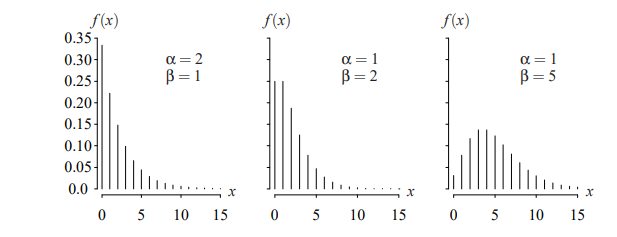
\includegraphics[width=1\textwidth]{image/泊松伽马分布.png}
  \caption{泊松伽马分布}
  \label{fig:example}
\end{figure}

 期望:

$$
E(X) = \alpha\beta
$$

 方差:

$$
D(X) = \alpha \beta + \alpha^{2}\beta
$$

 性质:

1. 做变换:$\alpha = (1 - p) / p, \beta = n$,就得到 Pascal 分布

\section{Zeta 分布(Zeta Distribution)}

 符号:$X \sim \text{Zeta}(\alpha)$

 概率函数:

$$
f(x) = \dfrac{1}{x^{\alpha}\sum\limits_{i = 1}^{+\infty}(1/i)^{\alpha}} \quad x = 1, 2, 3, ...
$$

\begin{figure}[H]
  \centering
  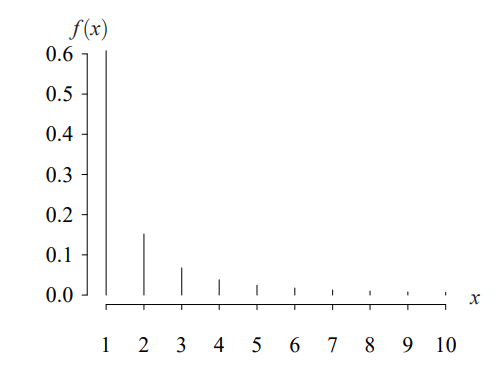
\includegraphics[width=0.7\textwidth]{image/Zeta分布.png}
  \caption{Zeta分布}
  \label{fig:example}
\end{figure}

 累计分布函数

$$
F(x) = P(X \leq x) = \dfrac{\sum\limits_{i = 1}^{x} (1/i)^{\alpha}}{\zeta(\alpha)} \quad x = 1, 2, ...
$$

 期望:

$$
E(X) = \dfrac{\zeta(\alpha - 1)}{\zeta(\alpha)}
$$

 方差:

$$
D(X) = \dfrac{\zeta(\alpha)\zeta(\alpha - 2) - \zeta(\alpha - 1)^{2}}{\zeta(\alpha)^{2}}
$$

\section{Zipf 分布(齐夫定律)}

 符号:$X \sim \text{Zipf}(\alpha, n)$

 概率函数:

$$
f(x) = \dfrac{1}{x^{\alpha}\sum\limits_{i = 1}^{n}(1 / i)^{\alpha}} \quad  x = 1, 2, 3, ..., n
$$

下面是 $\alpha = 1, n = 10$

\begin{figure}[H]
  \centering
  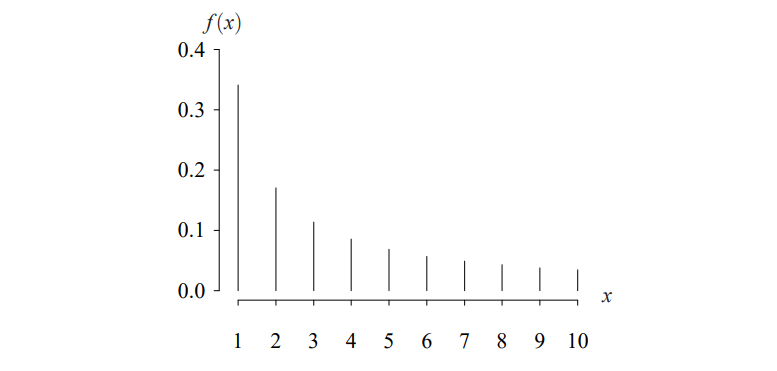
\includegraphics[width=1\textwidth]{image/齐夫分布.png}
  \caption{齐夫分布}
  \label{fig:example}
\end{figure}

我们记 $H_{n, \alpha} = \sum\limits_{i = 1}^{n} \left(\dfrac{1}{i}\right)^{\alpha}$

 期望:

$$
E(X) = \dfrac{H_{n, \alpha - 1}}{H_{n, \alpha}}
$$

 方差:

$$
D(X) = \dfrac{H_{n, \alpha - 2}H_{n, \alpha} - H_{n, \alpha}^{2}}{H_{n, \alpha}^{2}}
$$

 齐夫定律:

在自然语言的语料库里,一个单词出现的率与它在频率表里的排名成反比。所以,频率最高的单词出现的频率大约是出现频率第二位的单词的2倍,而出现频率第二位的单词侧是出现频率第四位的单词的2倍。这个定律被作为任何与幂定律概率分布有关的事物的参考。

 应用 or 遵循该定律的现象:

1. 英文单词或中文汉字的出现频率:不仅适用于语料全体,也适用于单独的一篇文章

2. 网页访问频率

3. 城镇人口与城镇等级的关系

4. 收入前3%的人的收入

5. 地震震级

6. 固体破碎时的碎片大小

\chapter{连续分布}

\section{均匀分布(Uniform Distribution)}

 符号:$X \sim U(a, b)$
 
 概率密度函数:

$$
f(x) = \begin{cases} \dfrac{1}{b - a} , a < x < b \\
0\end{cases}
$$

 分布函数:

$$
F(x) = \begin{cases}
\frac{x - a}{b - a}, &a < x < b \\
0,&x < a \\
1,&x > b
\end{cases}
$$

 期望:

$$
\begin{aligned}
E(X) &= \int_{-\infty}^{+\infty} x \cdot f(x) \mathrm{d}x \\
&= \int_{a}^{b} \dfrac{x}{b - a} \mathrm{d}x \\
&= \dfrac{a + b}{2}
\end{aligned}
$$

 方差:

$$
E(X^{2}) = \int_{a}^{b} \dfrac{x^{2}}{b - a} \mathrm{d}x
= \dfrac{a^{2}+ab + b^{2}}{3}
$$

$$
\begin{aligned}
D(X) &= E(X^{2}) - E(X)^{2} \\
&= \dfrac{a^{2}+ab + b^{2}}{3} - \left( \dfrac{a+b}{2}\right)^{2} \\
&= \dfrac{(b - a)^{2}}{12}
\end{aligned}
$$

 性质:

1. 一段有限区间上熵最大的分布族。

\section{指数分布(Exponential Distribution)}

指数分布一个很重要的特征就是无记忆性 $P(x > s | x > t) = P(x > s - t), s > t$ 。如果我们使用 x 表示等待的时间。那么这个式子的含义就是 未来我还需要等到多少时间和我已经等待了多长时间没有关系。

无记忆性的离散版本是 几何分布。

 符号:$X\sim E(\lambda)$

 概率密度函数:

$$
f(x) = \begin{cases}
\lambda e^{-\lambda x}, &x > 0 \\
\\
0, &x \leq 0
\end{cases}
$$

\subsection{指数分布推导:}

我们根据实际情况来考虑,如果一个产品的使用寿命是 T,分布函数是 $F(t)$,那么寿命大于 t 的概率为 $S(t) = 1- F(t)$

如果一个产品已经使用 t 时间,那么在 $(t, t + \Delta t)$ 这一段时间内,死亡的「风险」为:
$$
\lambda(t) = \lim\limits_{\Delta t \to 0} \dfrac{P(t \leq T \leq t + \Delta t)}{\mathrm{d}t \cdot S(t)} = \dfrac{f(t)}{S(t)} = -\dfrac{S'(t)}{S(t)} = -\dfrac{\mathrm{d}}{\mathrm{d}t}\ln(S(t))
$$
> 解释:因为我们首先需要活到这个时间,然后在这个时间段死亡,所以有 $S(t) \cdot \lambda(t) = p(T = t)$

我们称这个 $\lambda(t)$ 为风险函数(到这里还没有涉及到无记忆性,这个 $\lambda(t)$ 是一个普遍的风险函数)

如果我们要满足无记忆性,就要有 $\lambda(t) = \text{Const}$(也就是我们在每一个时间下「死亡」的概率都是等大的)

或者我们由「无记忆性」的直接式子推导:$P(T > s | T > t) = P(T > s - t) \Rightarrow P(t \leq T \leq t + \Delta t) = P(T < \mathrm{d}t) \cdot S(t)$ 也是得到 $\lambda(t) = \text{Const}$

所以有
$$
-\dfrac{\mathrm{d}}{\mathrm{d}t}\ln(S(t)) = \text{Const}
$$
解得 $F(t) = 1 - e^{-\text{Const} \cdot t}$

其中,$\text{Const}$ 表示每一个时间点死亡的风险大小,也就是每一个时间点死亡的概率大小。

 分布函数:

$$
F(x) = \begin{cases}
1 - e^{-\lambda x}, &x > 0 \\
0, &x \leq 0
\end{cases}
$$

 期望:

$$
\begin{aligned}
E(X) &= \int_{-\infty}^{+\infty} x \cdot f(x) \mathrm{d}x \\
&= \int_0^{+\infty} x \cdot \lambda e^{-\lambda x} \mathrm{d}x \\
&= x(-e^{-\lambda x})|_{0}^{+\infty} - \int_{0}^{+\infty} -e^{-\lambda x} \mathrm{d}x \\
&= \frac{1}{\lambda}
\end{aligned}
$$

 方差:

$$
\begin{aligned}
E(X^{2}) &= \int_0^{+\infty} x^{2} \cdot \lambda e^{-\lambda x} \mathrm{d}x \\
&= \int_0^{+\infty} x^{2} \mathrm{d}(-e^{-\lambda x}) \\
&= x^{2}(-e^{-\lambda x})|_{0}^{+\infty} + 2\int_0^{+\infty}xe^{-\lambda x} \mathrm{d}x \\
&= \frac{2}{\lambda^{2}}
\end{aligned}
$$

$$
D(X) = E(X^{2}) - E(X)^{2} = \frac{1}{\lambda^{2}}
$$

 性质:

1. 指数分布通常用来建模持续时间,只不过指数分布能够建模的持续时间具有比较特殊的性质,也就是所谓的“无记忆性”
2. 指数分布是在 $(0, +\infty)$ 支撑区间上熵最大的分布族。如果区间有限,那么熵最大的分布族就是均匀分布族,如果区间是全体实数,那么熵最大的分布族就是正态分布。

 应用:

1. 泊松分布、指数分布、二项分布、伯努利分布之间的关系:

   当 n 趋近于无穷大时,二项分布可以近似为泊松分布;当 $\lambda$ 趋近于无穷大
   时,泊松分布可以近似为正态分布;而指数分布则是泊松分布在连续时间上的推广,因此也与泊松
   分布有一定的联系。但是,这些分布之间的应用场景和特点是不同的,需要根据实际问题选择合适
   的分布模型。

\section{正态分布(高斯分布, Normal Distribution)}

 符号:$X\sim N(\mu, \sigma^{2})$

 概率密度函数:

$$
f(x) = \dfrac{1}{\sqrt{2\pi} \sigma}e^{-\frac{-(x-\mu)^{2}}{2\sigma^{2}}}(\mu \in R, \sigma > 0)
$$

 分布函数:

化为标准正态分布后查表应用。

 期望:

$$
\begin{aligned}
E(X) &= \int_{-\infty}^{+\infty} x \cdot \frac{1}{\sqrt{2 \pi} \sigma}e^{-\frac{-(x-\mu)^{2}}{2\sigma^{2}}} \mathrm{d}x \\
&=\int_{-\infty}^{+\infty}(x - \mu + \mu) \cdot \frac{1}{\sqrt{2\pi}\sigma}e^{-\frac{(x - \mu)^{2}}{2\sigma^{2}}} \mathrm{d}(x - \mu)\\
&= \int_{-\infty}^{+\infty} \frac{t}{\sqrt{2\pi}\sigma}e^{-\frac{t^{2}}{2\sigma^{2}}} \mathrm{d}t + \mu \int_{-\infty}^{+\infty}\frac{1}{\sqrt{2\pi}\sigma} e^{-\frac{(x - \mu)^{2}}{2\sigma^{2}}} \mathrm{d}x \\
&= 0 + \mu \\
&= \mu
\end{aligned}
$$

 方差:

$$
\begin{aligned}
D(X) &= \int_{-\infty}^{+\infty} x^{2} \cdot \frac{1}{\sqrt{2 \pi} \sigma}e^{-\frac{-(x-\mu)^{2}}{2\sigma^{2}}} \mathrm{d}x \\
&= \int_{-\infty}^{+\infty}(x - \mu)^{2} f(x) \mathrm{d}x + 2\mu \int_{-\infty}^{+\infty}x \cdot f(x) \mathrm{d}x - \mu^{2} \int_{-\infty}^{+\infty} f(x)\mathrm{d}x \\
&= \frac{1}{\sqrt{2\pi} \sigma}\int_{0}^{+\infty} \sqrt{t}e^{\frac{t}{2\sigma^{2}}} \mathrm{d}t + 2\mu^{2} - \mu^{2}\\
&= \sigma^{2}
\end{aligned}
$$

 性质:

1. 关于 $x = \mu$ 对称,其中 $\sigma^{2}$ 表示方差

2. $3\sigma$ 原则
   $P(\mu - 3\sigma \leq X \leq \mu + 3\sigma) = 0.9973$
   
3. 正态分布的线性组合仍然符合正态分布。

4. 标准正态分布:
   设 $Z = \dfrac{x - \mu}{\sigma}$,如果 $X \sim N(\mu, \sigma^{2})$,那么有 $Z \sim N(0, 1)$

 应用:

1. 统计学:正态分布在统计学中用于建模和分析许多自然现象,如测量误差、测试分数、人口身高、体重分布等。

3. 工程学:在工程学中,正态分布用于建模材料性质、产品尺寸、电子噪声等。

\subsection{ 正态分布公式推导:}

 情景建立以及基础推导

建设一个情景,我们想象我们是在向一个平面直角坐标系上朝着原点扔飞镖,会出现随机误差(我们扔的没有那么准)。

\begin{figure}[H]
  \centering
  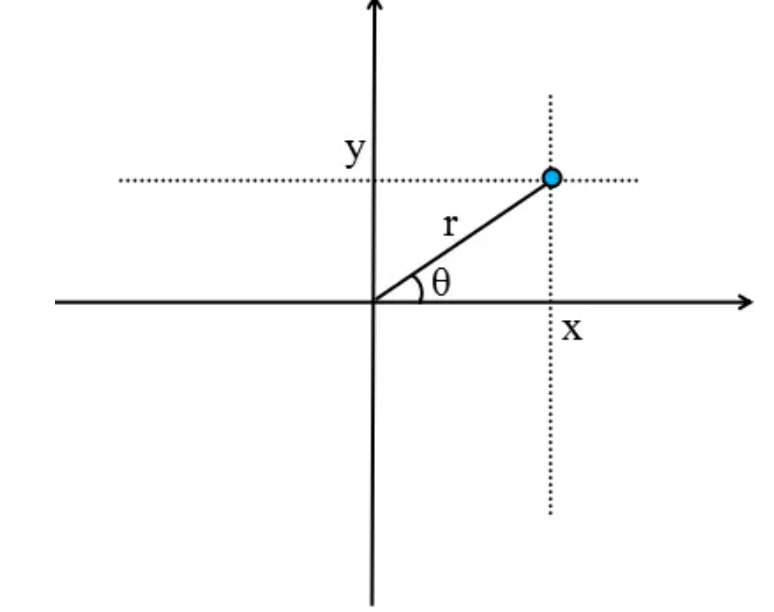
\includegraphics[width=0.6\textwidth]{image/正态分布推导.png}
  \caption{正态分布推导}
  \label{fig:example}
\end{figure}

飞镖出现在横坐标为 x 的位置的概率为 p(x),出现在纵坐标为 y 的位置的概率为 p(y)。

我们假设:

1. 误差与坐标系的方向无关(毕竟这个东西高度对称)
2. 大误差的可能性小于小误差的可能性(也就是偏离原点越远,我们越不可能扔到那里去)

所以落到 $(x,y)$ 位置的概率为 $g(x, y) = p(x) \cdot p(y)$

建立极坐标,有
$$
\dfrac{\mathrm{d}g(r)}{\mathrm{d}\theta} = 0
$$

整理后我们可以得到:

$$
\dfrac{p'(x)}{x \cdot p(x)} = \dfrac{p'(y)}{y \cdot p(y)} = \text{Const}
$$
解得,$p(x) = A \cdot e^{\frac{C}{2}x^{2}}$

因为 C 必须是一个负值,我们为了直观,将方程改写为 $p(x) = A\cdot e^{-\frac{k}{2}x^{2}}$

 确定常数 A:

因为函数 p 是概率分布,所以曲线下方的总面积必须为 1,所以有 $\int_{-\infty}^{+\infty}p(x)\mathrm{d}x = 1$

将 x y 两个方向的式子相乘,得到:
$$
\int_0^{+\infty}\int_0^{+\infty}e^{-\frac{k}{2}(x^{2} + y^{2})} \mathrm{d}x\mathrm{d}y = \dfrac{1}{4A^{2}}
$$

变换为极坐标形式求解左侧的积分,得到:$\dfrac{\pi}{2k}$,所以 $A = \sqrt{\dfrac{k}{2\pi}}$

 确定常数 k:

确定 A 我们是从概率密度函数的性质来得到的(每一个分布都有这个性质),但是对于某一个特殊的分布,总要有它「特别」不同于其他分布的性质,所以这就是我们后续推导正态分布公式需要使用的关系(毕竟我们需要创造一个分布不同于其他分布的性质条件),这就是数量性质,期望和方差。
$$
u = \int_{-\infty}^{+\infty} xp(x)\mathrm{d}x \\
\sigma^{2} = \int_{-\infty}^{+\infty}(x - u)^{2} p(x)\mathrm{d}x
$$

因为 $xp(x)$ 为基函数,所以 $u = 0$

$p(x)$对称,所以方差的式子可以写为:
$$
\begin{aligned}
\sigma^{2} &=\int_{-\infty}^{+\infty}x^{2}p(x)\mathrm{d}x \\
&= 2\int_0^{+\infty}x^{2}p(x)\mathrm{d}x \\
&= \dfrac{1}{k}
\end{aligned}
$$

所以,正态分布的最终形式就是
$$
p(x) = \dfrac{1}{\sqrt{2\pi}\sigma}e^{-\frac{(x - u)^{2}}{2\sigma^{2}}}
$$

 思考:

考虑为什么这样做可以推导出一元情况下的正态分布?

如果我们只是考虑一元一个维度下的情况,我们无法构建出它的方程。考虑一个平面给我们提供了更多的信息。

 其余推导方式:

我们也可以使用最大似然的方法或者信息熵的相关知识推导得到正态分布的公式。

1. [连续变量的最大熵分布 - 正态分布 - 知乎 使用信息熵的相关知识推导

2. [数学王子的壮举——高斯分布推导详解 - 知乎 最大似然的方式推导

\section{多元高斯分布(Multivariate Gaussian Distribution)}

 联合概率密度函数:

$$
p(x_1, x_2, ..., x_n) = \dfrac{1}{(2n)^{\frac{1}{2}}|\Sigma|^{\frac{1}{2}}} \cdot \exp(-\dfrac{1}{2}\left[(\vec{X} - \vec{\mu})^{T}\Sigma^{-1}(\vec{X} - \vec{u})\right])
$$

其中,$\Sigma$ 是协方差矩阵

 应用:
 
 多元高斯分布的性质和应用在统计学、机器学习、信号处理和贝叶斯推断等领域中都非常重要。

\section{混合高斯分布(Mixture of Gaussian Distributions)}


 应用:

混合高斯模型在许多领域中有广泛的应用,如模式识别、聚类分析、异常检测和图像分割。它允许建模复杂的数据分布,其中数据点可以由多个不同的分布生成,而不仅仅是单一的高斯分布。这使得混合高斯模型成为数据建模和分析中的强大工具。

\section{对数正态分布(Log-Normal Distribution)}

 符号:$X \sim \text{log-normal}(\alpha, \beta)$

 概率密度函数:

$$
f(x) = \dfrac{1}{x\beta \sqrt{2\pi}}e^{-\frac{1}{2}(\ln(x / \alpha) / \beta)^{2}}
$$

\begin{figure}[H]
  \centering
  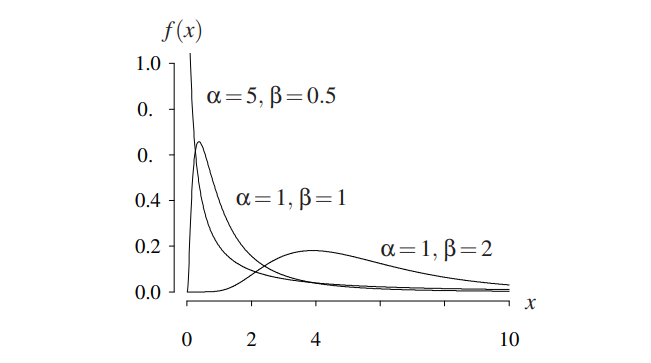
\includegraphics[width=1\textwidth]{image/对数正态分布.png}
  \caption{对数正态分布}
  \label{fig:example}
\end{figure}

 期望:

$$
E(X) = \alpha e^{\beta^2 / 2}
$$

 方差:

$$
D(X) = \alpha^{2}e^{\beta^{2}}(e^{\beta^{2}} - 1)
$$

 性质:

1. 对数正态性:对数正态分布的性质是,如果随机变量X服从对数正态分布,那么ln(X)(X的自然对数)将服从正态分布。这使得对数正态分布适用于描述正数随机变量的分布,如收入、股票价格、生物体的大小等。

2. 正偏分布:对数正态分布通常是右偏(正偏)的,这意味着它在对数尺度上呈现对称的正态分布形状。在原始尺度上,它可能具有长尾。

3. 均值和方差:对数正态分布的均值和方差取决于其参数。均值通常用μ表示,方差通常用$σ^2$表示,与正态分布参数不同。

4. 乘法性质:对数正态分布具有乘法性质,这意味着多个随机变量的对数正态分布之积仍然服从对数正态分布。这在金融学中用于模拟资产价格的变化以及在生物学中用于模拟生物体的生长。

 应用:

1. 金融学:对数正态分布经常用于模拟金融资产的价格变化,如股票价格和汇率。这对于风险管理、期权定价和模拟投资回报很有用。

2. 生物学:在生物学中,对数正态分布可用于描述生物体的大小、生长率和其他特征。例如,细胞大小、鱼的体长分布等。

\section{伽马分布(Gamma Distribution)}

 符号:$X \sim Ga(\alpha, \lambda)$

 概率密度函数:

$$
f(x) = \begin{cases}
\dfrac{\lambda^{\alpha}}{\Gamma(\alpha)} x^{\alpha - 1}e^{-\lambda x}, &x \geq 0\\
0 & x < 0
\end{cases}
$$

 期望:

$$
\begin{aligned}
E(X) &= \dfrac{\lambda^{\alpha}}{\Gamma(\alpha)}\int_{0}^{+\infty} x^{\alpha} e^{-\lambda x} \mathrm{d}x \\ &= \dfrac{\lambda^{\alpha}}{\Gamma(\alpha)} \int_{0}^{+\infty} \dfrac{t^{\alpha}}{\lambda ^{\alpha + 1}}e^{-t} \mathrm{d}t \\
&= \dfrac{\Gamma(\alpha  +1)}{\Gamma(\alpha) \cdot \lambda} \\
&= \frac{\alpha}{\lambda}
\end{aligned}
$$

 方差:

$$
\begin{aligned}
E(X^{2}) &= \int_{0}^{+\infty} x^{2} \cdot \dfrac{\lambda^{\alpha}}{\Gamma(\alpha)} x^{\alpha - 1}e^{-\lambda x} \mathrm{d}x \\
&= \dfrac{1}{\lambda^{2}\Gamma(\alpha)} \int_0^{+\infty} t^{\alpha+1}e^{-t}\mathrm{d}t \\
&= \dfrac{\alpha(\alpha + 1)}{\lambda^{2}}
\end{aligned}
$$

$$
D(X) = E(X^{2}) - E(X)^{2}  = \dfrac{\alpha}{\lambda^{2}}
$$

 性质:

1. $\alpha  = 1$ 的时候,伽马分布与指数分布之间的关系就建立起来了,有 $Ga(1, \lambda ) = E(\lambda)$

2. 当 $\alpha = \dfrac{n}{2}, \lambda = \dfrac{1}{2}$ 的时候,伽马分布和卡方分布之间的关系就建立起来了,有 $Ga(\dfrac{n}{2}, \dfrac{1}{2}) = \mathcal{X}^{2}(n)$

3. 伽马分布的可加性。
   如果有 $X \sim \Gamma(\alpha_1, \lambda), Y \sim \Gamma(\alpha_2, \lambda)$,并且 X 和 Y 相互独立,则有 $Z = X + Y \sim \Gamma(\alpha_1 + \alpha_2, \lambda)$

 应用:

1. 通信工程:在通信工程中,伽马分布可以用于建模通信信号的功率和噪声,以便进行信号处理和通信系统设计。

2. 自然科学:在物理学和工程学领域,伽马分布通常用于描述粒子的能量分布、原子核的衰变时间和电子束的强度分布。

3. 排队理论:伽马分布可以用于排队理论,描述顾客到达和服务时间的分布,以分析和优化排队系统的性能。

4. 机器学习:在深度学习和神经网络中,伽马分布有时被用于建模损失函数的分布,特别是在回归问题中。


\section{对数伽马分布(Log-Gamma Distribution)}
 符号:$X \sim \text{log-gamma}(\alpha, \beta)$

 概率密度函数:

$$
f(x) = \dfrac{e^{\beta x}e^{-e^{x} / a}}{\alpha^{\beta}\Gamma(\beta)} -\infty < x < +\infty
$$
\begin{figure}[H]
  \centering
  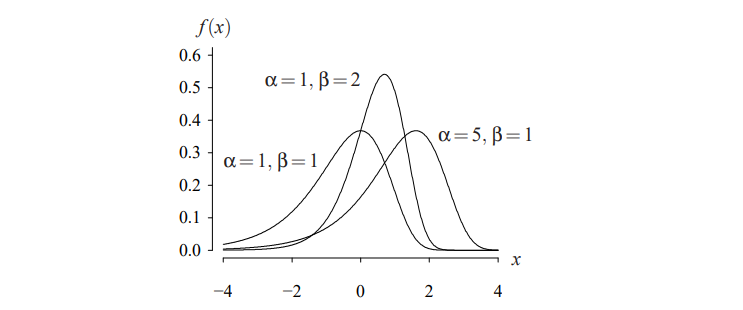
\includegraphics[width=1\textwidth]{image/对数伽马分布.png}
  \caption{对数伽马分布}
  \label{fig:example}
\end{figure}

性质:

1. 正数值数据分布: 对数伽马分布通常用于建模正数值数据,如收入、成交金额、寿命、失效时间等。由于其在正实数范围内定义,适用于非负随机变量。

2. 形状参数和尺度参数: 对数伽马分布有两个参数,$\alpha$ 和 $\beta$,分别影响分布的形状和尺度。较大的 $\alpha$ 值表示分布更陡峭,而较大的 $\beta$ 值表示分布更平缓。

3. 自然对数转换: 这个分布之所以称为"对数伽马",是因为随机变量 $X$ 经过自然对数转换(取对数)后,它会变成伽马分布。

4. 尾部行为: 对数伽马分布的尾部通常是重尾分布,意味着它可以很好地捕捉尾部极端事件的概率。

应用:

1. 金融建模: 对数伽马分布可用于建模金融市场中的资产价格波动、收益率分布和风险管理。它能够帮助分析收益分布,尤其是在考虑风险和波动性时。

2. 生存分析: 在生物统计学和医学领域,对数伽马分布用于描述寿命或失效时间的分布。这对于分析产品的寿命、生存概率和可靠性非常有用。

3. 可靠性工程: 对数伽马分布在可靠性工程中用于建模产品的寿命分布和故障分布。它有助于预测设备的寿命和维护计划。

4. 经济数据分析: 经济学家和研究人员经常使用对数伽马分布来描述经济数据,如收入分布、消费数据、通货膨胀率等。

5. 模拟和推断: 对数伽马分布也用于生成模拟数据,进行参数估计和假设检验。它可以与最大似然估计等统计方法结合使用。

\section{贝塔分布(Beta Distribution)}

符号:$X \sim \Beta(\alpha, \beta)$

 概率密度函数:

$$
f(x) = \begin{cases}
\dfrac{1}{\Beta(\alpha, \beta)} x^{\alpha - 1}(1-x)^{\beta - 1}, 0 < x < 1 \\
0
\end{cases}
$$

分布函数:

期望:

\[
\begin{aligned}
E(X) &= \int_0^{1}x \cdot \frac{1}{\Beta(\alpha, \beta)} x^{\alpha - 1}(1-x)^{\beta - 1} \mathrm{d}x \\
&= \frac{\Beta(\alpha + 1, \beta)}{\Beta(\alpha, \beta)} \int_0^{1}\frac{1}{\Beta(\alpha + 1, \beta)} x^{(\alpha + 1) - 1}(1-x)^{\beta - 1} \mathrm{d}x \\
&= \frac{\Gamma(\alpha + 1)\Gamma(\beta)}{\Gamma(\alpha + \beta + 1)} \cdot \frac{\Gamma(\alpha + \beta)}{\Gamma(\alpha)\Gamma(\beta)} \\
&= \frac{\alpha}{\alpha + \beta}
\end{aligned}
\]

方差:

\[
\begin{aligned}
E(X^{2}) &= \int_0^{1} \dfrac{1}{\Beta(\alpha, \beta)}x^{(\alpha + 2) - 1}(1 - x)^{\beta - 1} \mathrm{d}x \\
&= \dfrac{\Beta(\alpha + 2, \beta)}{\Beta(\alpha, \beta)} \\
&= \dfrac{\alpha(\alpha + 1)}{(\alpha + \beta)(\alpha + \beta + 1)}
\end{aligned}
\]

$$
D(X) = E(X^{2}) - E(X)^{2} = \dfrac{\alpha \beta}{(\alpha + \beta)^{2}(\alpha + \beta + 1)}
$$

 性质:

1. $Beta(1, 1) = U(0, 1)$

\section{威布尔分布(韦伯分布,Weibull Distribution)}

概率密度函数:

$$
f(x;\lambda, k) = \begin{cases}
\dfrac{k}{\lambda}(\dfrac{x}{\lambda})^{k - 1}e^{-(\dfrac{x}{\lambda})^k}, &x \geq 0 \\
0, &x < 0
\end{cases}
$$

其中,x 是随机变量,$\lambda > 0$ 是比例系数(scale parameter),$k > 0$ 是形状参数(shape parameter)。显然,它的累计分布函数是扩展的指数分布函数。

 期望:

$$
E(X) = \lambda \Gamma(1 + \dfrac{1}{k})
$$

 方差:

$$
D(X) = \lambda^{2}\left[\Gamma(1 + \dfrac{2}{k}) - \Gamma^{2}(1 + \dfrac{1}{k})\right]
$$

 应用:

威布尔分布在可靠性工程中被广泛应用。

1. 研究生产过程和运输时间关系

2. 预测天气

3. 可靠性和失效分析

4. 雷达系统

5. 对接受的杂波信号依分布建模

6. 量化寿险模型的重复索赔

7. 描述风速分布

\section{瑞利分布(Rayleigh Distribution)}

 含义:

当一个随机二维向量的两个分量呈独立的、均值为0,有着相同的方差的呈瑞利分布。

 推导:

复高斯分布就是实部和虚部都满足高斯分布的一种分布,表示为 $ Z= X + iY$,其中 $X\sim N(\mu_x, \sigma_x^{2}), Y \sim N(\mu_y, \sigma_y^{2})$

对于一个实部和虚部都是零均值独立同分布的复高斯分布 Z = X + iY

瑞利分布就是两个垂直分量服从独立且均值为0,标准差相同的高斯分布叠加之后的模。换句话说,复高斯分布的模服从瑞利分布。

\begin{figure}[H]
  \centering
  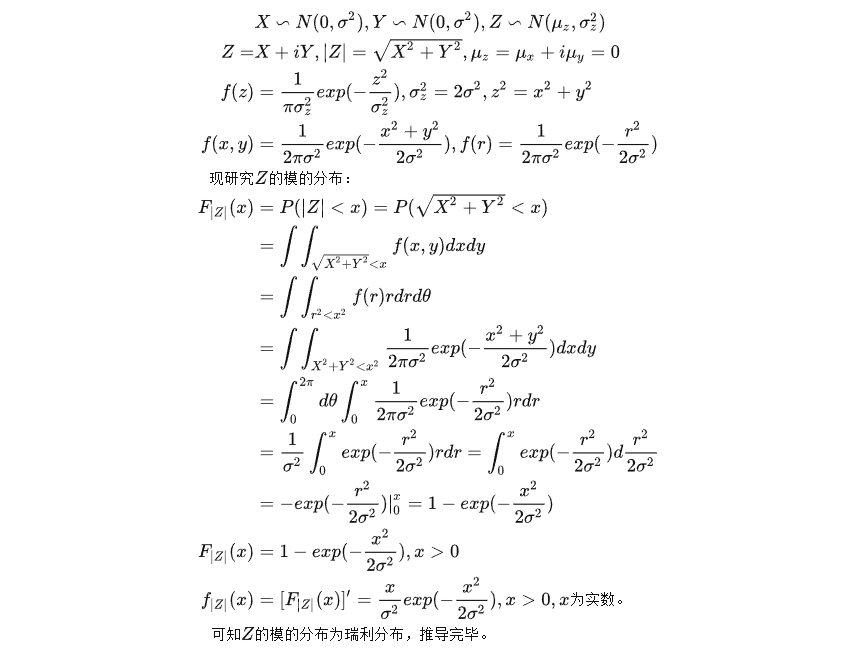
\includegraphics[width=1\textwidth]{image/瑞利分布.png}
  \caption{瑞利分布}
  \label{fig:example}
\end{figure}

\section{柯西分布(柯西-洛伦兹分布,Cauchy Distribution)}

 符号:$X \sim \text{Cauthy}(a, \alpha)$

 概率密度函数:

$$
f(x) = \dfrac{1}{\alpha\pi[1 + ((x - a) / \alpha)^{2}]} \quad \quad -\infty < x < +\infty
$$

\begin{figure}[H]
  \centering
  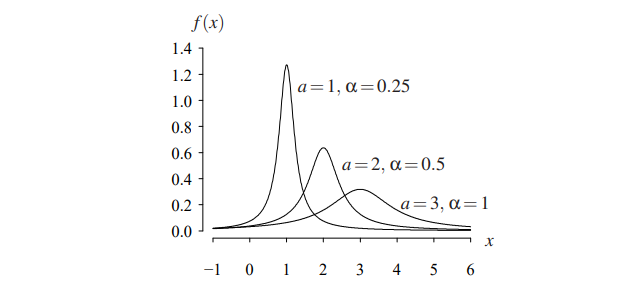
\includegraphics[width=1\textwidth]{image/柯西分布.png}
  \caption{柯西分布}
  \label{fig:example}
\end{figure}

 由来推导:

柯西分布描述了以随机角度倾斜的线段切割 x 轴的水平距离分布。

\begin{figure}[H]
  \centering
  
\includegraphics[width=1\textwidth]{image/柯西分布推导.png}
  \caption{柯西分布推导}
  \label{fig:example}
\end{figure}
$$
\tan(\theta) = \dfrac{x}{b} \\
\theta = \arctan{\dfrac{x}{b}} \\
\mathrm{d}\theta = \dfrac{1}{1 + \frac{x^{2}}{b^{2}}} \dfrac{\mathrm{d}x}{b}
$$

所以可以使用 $\dfrac{\mathrm{d}\theta}{\pi} = \dfrac{1}{\pi} \dfrac{b\mathrm{d}x}{b^2 + x ^{2}}$ 来计算关于 x 的分布。
$$
\int_{-\frac{\pi}{2}}^{\frac{\pi}{2}} \dfrac{\theta}{\pi} = 1 \Rightarrow \int_{-\infty}^{+\infty} \dfrac{1}{\pi} \dfrac{b \mathrm{d}x}{b^2 + x^{2}} = 1
$$

所以,$P(X = x) = \dfrac{1}{\pi} \dfrac{b}{(x - m)^{2} + b^2}$

 分布函数:

$$
F(x) = P(X \leq x) = \dfrac{1}{2\pi}\left(\pi - 2\arctan(\dfrac{a - x}{\alpha})\right) \quad -\infty < x < +\infty
$$

 期望:

不存在

 方差:
不存在

 应用:

1.  柯西分布,也称为柯西-洛伦兹分布或洛伦兹分布,是描述共振行为的连续分布。它还描述了以随机角度倾斜的线段切割 x 轴的水平距离分布。

2. 在量子世界,粒子和粒子距离很远,比如,电子到原子核的距离,就好比一个汽车到三千公里外的一个城市距离,因此,要显著描述电子的位置分布,只能是柯西-洛伦兹分布,不能用高斯分布刻画,因为高斯分布尺度不够,信号太弱,噪声将把电子的电磁能量淹没,模型无效。

 性质:

1.  柯西分布的取值范围非常广,很大的值也有一定概率取到,因而柯西分布也称为heavy-tail distribution。并且相比于gaussian,概率密度的最大取值只有0.1,就是x=0的那个地方。


\section{拉普拉斯分布(双指数分布,Laplace Distribution)}

 符号:$X \sim \text{Laplace}(\alpha_1, \alpha_2)$

 概率密度函数:

$$
f(x) = \begin{cases}
\dfrac{1}{\alpha_1 + \alpha_2}e^{-\frac{x}{\alpha_1}}, &x < 0 \\
\dfrac{1}{\alpha_1 + \alpha_2}e^{-\frac{x}{\alpha_2}}, & x \geq 0
\end{cases}
$$

The Laplace distribution is an alternative to the normal distribution with heavier tails. The probability density function for three different parameters settings is illustrated below.

\begin{figure}[H]
  \centering
  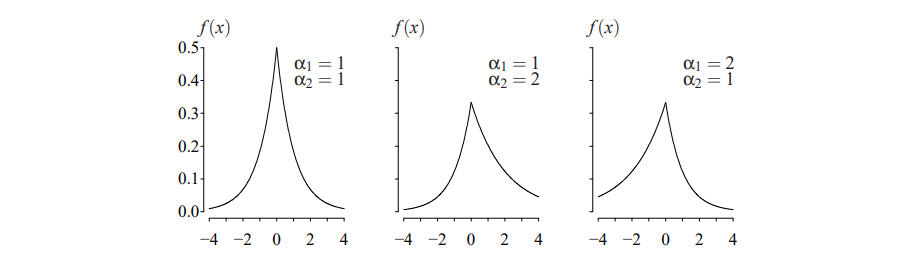
\includegraphics[width=1\textwidth]{image/拉普拉斯分布.png}
  \caption{拉普拉斯分布}
  \label{fig:example}
\end{figure}

 分布函数:

$$
F(x) = P(X \leq x) = \begin{cases}
\dfrac{\alpha_1}{\alpha_1 + \alpha_2}e^{-\frac{x}{\alpha_1}} &x < 0 \\
1 - \dfrac{\alpha_2}{\alpha_1 + \alpha_2}e^{-\frac{x}{\alpha_2}}&x \geq 0
\end{cases}
$$

 期望:

$$
\begin{aligned}
E(X) &= \int_{-\infty}^{0} x \cdot f(x)\mathrm{d}x + \int_0^{+\infty} x \cdot f(x) \mathrm{d}x\\
&= \alpha_2 - \alpha_1
\end{aligned}
$$

 方差:

$$
\begin{aligned}
D(X) &= \int_{-\infty}^{0} x^2 \cdot f(x)\mathrm{d}x + \int_0^{+\infty} x^2 \cdot f(x) \mathrm{d}x\\
&= \alpha_1^{2} + \alpha_2^{2}
\end{aligned}
$$

 性质:

1. 可看作两平移指数分布背靠背拼接在一起,因此又称双指数分布 (Double exponential distribution)
2. 拉普拉斯分布的图像形式和正态分布很像。
   不过拉普拉斯分布是「尖峰」,而正态分布是「平顶」。

 应用:

1. 机器学习:在机器学习中,拉普拉斯分布经常用于贝叶斯估计和参数估计。它在贝叶斯推断中常用作先验分布,因为它对模型参数的稀疏性具有天然的建模能力。

2. 图像分析:在计算机视觉和图像处理中,拉普拉斯分布用于描述图像中像素强度值的分布,以进行边缘检测、图像增强和纹理分析。

3. 统计分析:拉普拉斯分布可用于建模具有长尾数据或离群值的情况。它在异常检测和统计分析中用于识别和处理离群值。

4. 通信工程:在通信工程中,拉普拉斯分布用于建模通信信道中的噪声和失真,以进行信号处理和通信系统设计。


\section{玻尔兹曼分布(Boltzmann Distribution)}

玻尔兹曼分布(Boltzmann Distribution)是一种在统计物理学和热力学中广泛使用的分布,用于描述粒子在不同能级(能量状态)上的分布概率。

 性质:

1. 指数分布:玻尔兹曼分布的概率密度函数具有指数形式,通常表示为$P(E) = (1/Z)  e^(-E / kT)$,其中E是能量,T是温度,k是玻尔兹曼常数,Z是配分函数,它是用于归一化分布的常数。

2. 能级依赖:玻尔兹曼分布的概率分布取决于能级E和温度T之间的关系。较高的温度使得较高能级的状态更有可能被占据。

3. 温度影响:温度对玻尔兹曼分布的形状和性质产生显著影响。高温下,分布更加平坦,而在低温下,分布更加尖锐。

4. 热平衡:在热平衡条件下,玻尔兹曼分布描述了粒子分布在不同能级上的均衡状态,其中能级的占据概率与温度有关。

 应用:

1. 统计物理学:玻尔兹曼分布是统计物理学中的基本概念,用于描述粒子在能级上的分布。它在描述气体分子的速度分布、原子在固体中的能级分布等方面有广泛应用。

2. 热力学:在热力学中,玻尔兹曼分布用于解释气体和固体中粒子的热运动,以及描述温度和能量之间的关系。

3. 化学:在化学反应动力学中,玻尔兹曼分布可以用于理解反应速率和活化能之间的关系,以及在不同温度下反应的速率。

4. 天文学:在天文学中,玻尔兹曼分布可以用于分析恒星内部的能级分布和温度分布,从而理解恒星的演化和性质。

5. 工程学:在工程学中,玻尔兹曼分布可以用于建模材料中原子或分子的热运动,以帮助设计和分析材料的性能。

\section{幂律分布(Power Distribution)}

 符号:$X\sim \text{Power}(\alpha, \beta)$

 概率密度函数:

$$
f(x) = \dfrac{\beta x^{\beta - 1}}{\alpha^{\beta}} \quad \quad 0 < x < \alpha
$$

\begin{figure}[H]
  \centering
  
\includegraphics[width=1\textwidth]{image/幂律分布.png}
  \caption{幂律分布}
  \label{fig:example}
\end{figure}

 分布函数:

$$
F(x) = P(X \leq x) = \dfrac{x^{\beta}}{\alpha^{\beta}}
$$

 期望:

$$
E(X) = \dfrac{\alpha \beta}{1 + \beta}
$$

 方差:

$$
D(X) = \dfrac{\alpha^{2}\beta}{(2 + \beta)(1 + \beta)^{2}}
$$

 性质:

不适用中心极限定理:幂律分布不满足中心极限定理,因此它们不具有正态分布的性质。

 应用:

1. 社交网络和互联网:在社交网络中,幂律分布可以用于描述节点的度分布,其中少数节点具有极高的连接度。在互联网中,幂律分布也可用于描述网页的入站链接分布和流行度分布。

2. 城市规模分布:Zipf's Law 是一种特殊的幂律分布,用于描述城市的人口规模分布,其中少数大城市拥有多数人口,而大多数城市人口相对较少。

3. 科学文献引用:科学文献引用网络中,幂律分布通常用于描述论文被引用的频率分布。少数论文会被广泛引用,而大多数论文只被引用很少次。

4. 金融领域:在金融市场中,资产价格的涨跌通常遵循幂律分布,其中大幅上涨或下跌的情况出现频率较低,但具有重要影响。

5. 自然现象:在自然界中,地震、火山爆发、气象事件和生物物种的分布等现象也可以遵循幂律分布。

6. 网络科学:在网络科学中,幂律分布用于描述网络中节点的度分布、网页的点击率分布和互联网流量的分布。

\section{三角分布(Standard Triangular Distribution)}

 符号:$X \sim \text{Triangular}(-1, 1, 1)$

 概率密度函数:

$$
f(x) = \begin{cases}
x + 1, &-1 < x < 0 \\
1 - x, & 0 \leq x < 1
\end{cases}
$$

\begin{figure}[H]
  \centering
  
\includegraphics[width=1\textwidth]{image/三角分布.png}
  \caption{三角分布}
  \label{fig:example}
\end{figure}

 分布函数:

$$
F(x) = \begin{cases}
\frac{1}{2}x^{2} + x + \frac{1}{2}, &-1 < x < 0 \\
-\frac{1}{2}x^{2} + x + \frac{1}{2}, &0 \leq x < 1
\end{cases}
$$

 期望:

$$
E(X) = 0
$$

 方差:

$$
D(X) = \dfrac{1}{6}
$$

更一般的,三角形分布是底限为 a,众数为 c,上限为 b 的连续概率分布。

$$
f(x|a, b, c) = \begin{cases}
\dfrac{2(x - a)}{(b - a)(c - a)} \quad a \leq x \leq c \\
\\
\dfrac{2(b - x)}{(b - a)(b - c)} \quad c \leq x \leq b
\end{cases}
$$

\begin{figure}[H]
  \centering
  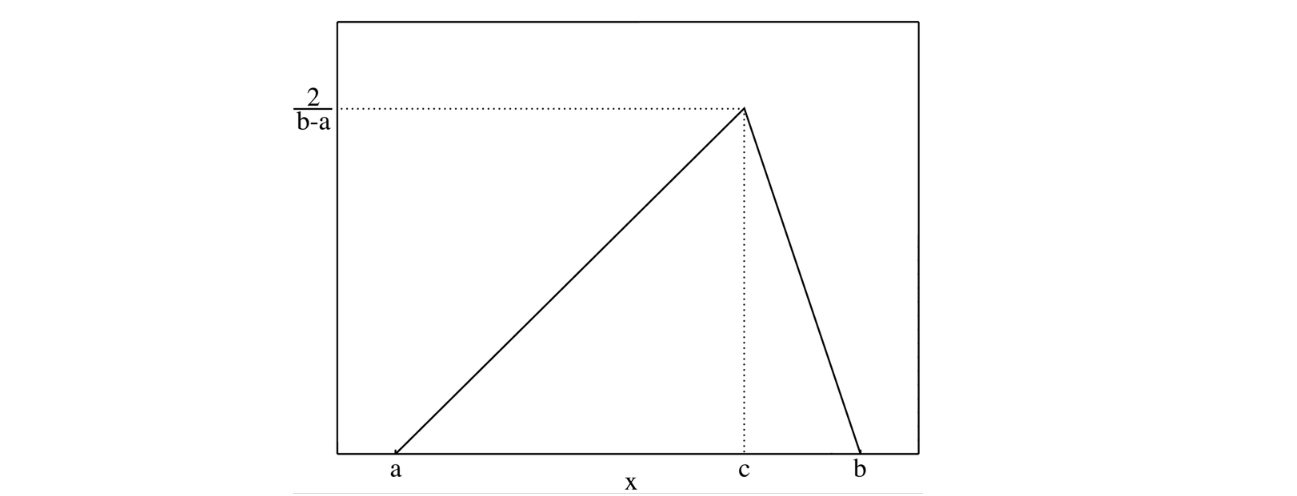
\includegraphics[width=1\textwidth]{image/三角分布进阶.png}
  \caption{一般三角分布}
  \label{fig:example}
\end{figure}

\section{逻辑斯谛分布(增长分布, Log-Logistic Distribution)}

 逻辑斯谛函数:

逻辑斯蒂函数(Loglogistic Function)一般指函数 $N(t) = \dfrac{e^{Z}}{1 + e^{Z}}$,其中 $Z = \alpha + \beta t$

这个函数是 Logistic 微分方程的解,后者最初目的是作为描述人口增长的模型。更确切地说,是 Malthus 人口模型的修正。此后,Logistic函数又被广泛运用在了概率论、机器学习等领域;而由Logistic微分方程衍生出的Logistic差分方程中人们发现了神奇的混沌现象,并催化出了《周期三意味着混沌》这篇混沌理论的“开山之作”以及费根鲍姆常数。

逻辑斯蒂函数就是微分方程 $\dfrac{\mathrm{d}N(t)}{\mathrm{d}t}= \dfrac{rN(K - N)}{K}$ 的解。

 符号:$X \sim \text{loglogistic}(\lambda, \kappa)$

 概率密度函数:

$$
f(x) = \dfrac{\lambda\kappa(\lambda\kappa)^{\kappa - 1}}{(1 + (\lambda x)^{\kappa})^{2}} \quad x > 0
$$

\begin{figure}[H]
  \centering
  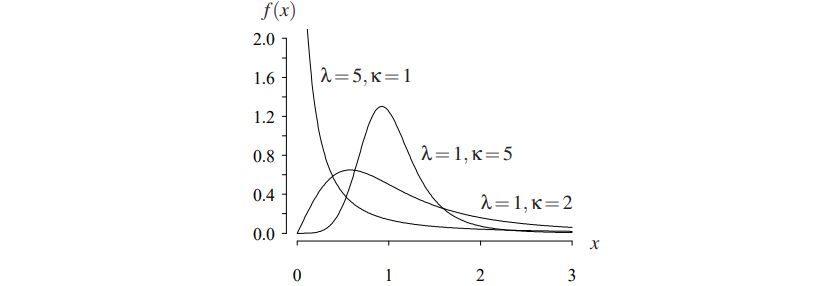
\includegraphics[width=1\textwidth]{image/逻辑斯谛分布.png}
  \caption{逻辑斯谛分布}
  \label{fig:example}
\end{figure}

 分布函数:

$$
F(x) = P(X <= x) = \dfrac{(\lambda x)^{\kappa}}{1 + (\lambda x)^{\kappa}}  \quad x > 0
$$

 期望:

$$
\begin{aligned}
E(X) &= \int_0^{+\infty} x \cdot f(x) \mathrm{d}x \\
&= \dfrac{1}{\lambda} \int_0^{+\infty}\dfrac{m^{\frac{1}{k}}}{(1+m)^{2}} \mathrm{d}m \\
&= \dfrac{1}{\kappa \lambda} \cdot \dfrac{\pi}{\sin (\frac{\pi}{\kappa})} \\
&= \dfrac{\pi}{\kappa \lambda(\sin (\frac{\pi}{\kappa})}
\end{aligned}
$$

其中,计算的时候可以使用留数定理。

 方差:

$$
D(X) = \dfrac{\pi \left(2\kappa(1 - \cos (\frac{\pi}{\kappa})^{2}) + \pi\sin(\frac{\pi(\kappa + 2)}{\kappa}) \right)}{\left(\sin (\frac{\pi(\kappa + 2)}{\kappa}) \right)\left( \cos(\frac{\pi}{\kappa})^{2} - 1\right)(\lambda \kappa)^{2}}
$$

\section{逻辑分布(Logistic Distribution)}

 符号:$X \sim \text{logistic}(\lambda, \kappa)$

 概率密度函数:

$$
f(x) = \dfrac{\lambda^{\kappa}\kappa e^{\kappa x}}{(1 + (\lambda e^{x})^{\kappa})^{2}} \quad -\infty < x < +\infty
$$

\begin{figure}[H]
  \centering
  
\includegraphics[width=1\textwidth]{image/逻辑分布.png}
  \caption{逻辑分布}
  \label{fig:example}
\end{figure}

 分布函数:

$$
F(x) = P(X \leq x) = \dfrac{\lambda^{\kappa}e^{\kappa x}}{1 + \lambda^{\kappa}e^{x}} \quad -\infty < x < +\infty
$$

 期望:

$$
E(X) = -\ln \lambda
$$

 方差:

$$
D(X) = \dfrac{\pi ^{2}}{3\kappa^{2}}
$$

 性质:

1. 最大熵分布:在信息论中,逻辑分布是熵最大的连续分布之一,因此它在最大熵原理的背景下具有重要性。

2. 广义线性模型:逻辑分布是广义线性模型(GLM)中的一种重要分布,特别用于二元分类问题,如逻辑回归,其中它用于建模事件发生的概率。

3. S-形曲线:逻辑分布的概率密度函数具有S形曲线,这使得它在模拟二元随机事件的概率分布中非常有用。这种曲线的形状使逻辑分布常用于建模生长、饱和和饱和增长现象。

 应用:

1. 生物学:逻辑分布用于建模生物学中的生长和饱和现象,如细胞增长、食物消耗和酶反应速率。

2. 医学统计:在医学统计学中,逻辑分布用于建模疾病发病率、药物吸收、生存分析和临床试验中的治疗效果。

3. 机器学习:逻辑分布广泛应用于分类问题,特别是逻辑回归是用于二元和多元分类的重要机器学习算法。

4. 金融学:在金融领域,逻辑分布用于建模金融风险、市场波动性和金融事件的概率。

5. 社会科学:逻辑分布可用于建模社会科学中的事件发生概率,如政治选举结果、市场份额预测和社会趋势。

\section{t 分布(T Distribution)}

如果 $X\sim N(0, 1), Y \sim \chi^{2}(n)$,则有 $Z = \dfrac{X}{\sqrt{\frac{Y}{n}}} \sim t(n)$

 概率密度函数:

$$
\begin{aligned}
f(z) =\dfrac{\Gamma(\frac{n + 1}{2})}{\sqrt{n\pi}\Gamma(\frac{n}{2})}\left(\dfrac{z^{2}}{n} + 1\right)^{-\frac{n + 1}{2}}
\end{aligned}
$$

 推导:

做变换:

$$
\begin{aligned}
\begin{cases}
u = \dfrac{X}{\sqrt{\frac{Y}{n}}} \\
\\
v = Y
\end{cases}
\end{aligned}
$$

所以有反函数:

$$
\begin{cases}
X = u\sqrt{\dfrac{v}{n}} \\
\\
Y = v
\end{cases}
$$

雅可比行列式是:

$$
|J| = \begin{vmatrix}
\dfrac{\partial X}{\partial u} & \dfrac{\partial X}{\partial v} \\
\\
\dfrac{\partial Y}{\partial u} & \dfrac{\partial Y}{\partial V}
\end{vmatrix}
$$

所以原问题的分布函数变为:

$$
\begin{aligned}
\iint\limits_{A}f(x,y)\mathrm{d}x\mathrm{d}y &= \iint\limits_{B}f(x(u, v),y(u, v)) |J| \mathrm{d}u \mathrm{d}v \\
&= \int_{-\infty}^{z}\int_{0}^{+\infty}f_X(u\sqrt{\dfrac{v}{u}})f_Y(v) (\dfrac{v}{n})^{-\frac{1}{2}} \mathrm{d}u \mathrm{d}v \\

\end{aligned}
$$

有

$$
\begin{aligned}
f_X(x) &= \dfrac{1}{\sqrt{2\pi}}e^{-\frac{x^{2}}{2}} \\
f_Y(y) &= \dfrac{1}{2^{\frac{n}{2}}\Gamma(\frac{n}{2})}y^{\frac{n}{2}- 1}e^{-\frac{y}{2}}
\end{aligned}
$$

所以:

$$
\begin{aligned}
F(Z) &= \int_{-\infty}^{z}\int_0^{+\infty} \dfrac{1}{\sqrt{2\pi}}e^{-\frac{1}{2}u^{2}\frac{v}{n}} \dfrac{1}{2^{\frac{n}{2}}\Gamma(\frac{n}{2})}v^{\frac{n}{2} - 1} e^{-\frac{v}{2}}(\dfrac{v}{n})^{-\frac{1}{2}} \mathrm{d}v\mathrm{d}u \\
&= \int_{-\infty}^{z}\dfrac{1}{\sqrt{n\pi}\sqrt{2}}\dfrac{1}{2^{\frac{n}{2}} \Gamma(\frac{n}{2})} \int_0^{+\infty}e^{-\frac{1}{2}u^{2}\frac{v}{n} - \frac{v}{2}}v^{\frac{n - 1}{2}} \mathrm{d}u \mathrm{d}v
\end{aligned}
$$

 期望:

$$
E(X) = 0
$$

 方差:

$$
V(X) = \dfrac{n}{n - 2}
$$

 性质:
 
1. 形状和对称性: t分布具有钟形曲线形状,类似于正态分布,但尾部较宽。t分布是对称的,围绕均值对称。

2. 参数: t分布的参数是自由度(degrees of freedom),通常用字母ν表示。自由度决定了t分布的形状,自由度越大,分布越接近正态分布。

3. 尾部厚度: t分布的尾部比正态分布厚,这意味着它对极端值的容忍性更强,因此更适合处理小样本数据。

4. 中心极限定理: 当样本容量足够大时(通常大于30),t分布近似于正态分布。这是因为根据中心极限定理,大样本均值的分布趋向于正态分布。

5. 样本平均值的分布: t分布用于估计总体均值的抽样分布,特别是在小样本情况下。它可以帮助进行区间估计和假设检验。

 应用:

1. 小样本推断: t分布广泛用于小样本情况下的统计推断。例如,在小样本情况下,使用t分布来进行样本均值的区间估计和假设检验,如t检验。

2. 置信区间估计: t分布用于计算均值的置信区间。给定一个样本均值和样本标准差,t分布可用于估计总体均值的区间范围,通常使用t分布的百分位数。

3. 假设检验: t分布在假设检验中非常有用,特别是当总体标准差未知时。它可以用于检验总体均值是否等于特定值,或者不同样本均值之间是否存在显著性差异。

4. 回归分析: t统计量在回归分析中常用于检验回归系数的显著性,以确定自变量是否对因变量产生显著影响。

5. 贝叶斯分析: t分布也可以与贝叶斯统计学结合使用,用于建立贝叶斯模型中的后验分布。

\section{F 分布(F Distribution)}

F 分布也被称为「方差比分布(Variance Ratio Distribution)」和「Fisher-Snedecor Distribution」。

设 $U \sim \chi^{2}(n_1), V \sim \chi^{2}(n_2)$,并且 U 和 V 相互独立,则称随机变量 $F = \dfrac{U / n_1}{V / n_2}$ 服从自由度为 $(n_1, n_2)$ 的 F 分布

 概率密度函数:

$$
f(z) = \dfrac{\Gamma(\frac{n_1 + n_2}{2})(\frac{n_1}{n_2})^{\frac{n_1}{2}}z^{\frac{n_1}{2} - 1}}{\Gamma(\frac{n_1}{2})\Gamma(\frac{n_2}{2})\left[1 + \frac{n_1}{n_2}z\right]^{\frac{n_1 + n_2}{2}}}
$$

 推导:

$\text{lemma1}:$
$$
f_{\frac{Y}{X}}(z) = \int_{-\infty}^{+\infty}|x|f(x, xz)\mathrm{d}x
$$

$\text{lemma2}:$
$$
f_{aX + b} = \dfrac{1}{|a|}f_X(\dfrac{y - b}{a}) \quad a \neq 0
$$

所以我们可以得到 $Y = \dfrac{U}{n_1}, X = \dfrac{V}{n_2}$ 的概率密度函数为:

$$
f_Y(y) = \dfrac{(\frac{n_1}{2})^{\frac{n_1}{2}}}{\Gamma(\frac{n_1}{2})}y^{\frac{n_1}{2} - 1}e^{-\frac{n_1y}{2}} \quad y > 0
$$

$$
f_X(x) = \dfrac{(\frac{n_2}{2})^{\frac{n_2}{2}}}{\Gamma(\frac{n_2}{2})}y^{\frac{n_2}{2} - 1}e^{-\frac{n_2y}{2}} \quad x > 0
$$

$$
\begin{aligned}
f_F(z) &= f_{\frac{Y}{X}}(z) \\
&= \int_0^{+\infty} xf(x, xz) \mathrm{d}x \\
&= \int_0^{+\infty} xf_Y(xz)f_X(x) \mathrm{d}x \\
&= \int_0^{+\infty} x \dfrac{(\frac{n_1}{2})^{\frac{n_1}{2}}}{\Gamma(\frac{n_1}{2})}(xz)^{\frac{n_1}{2} - 1}e^{-\frac{n_1y}{2}} \cdot  \dfrac{(\frac{n_2}{2})^{\frac{n_2}{2}}}{\Gamma(\frac{n_2}{2})}y^{\frac{n_2}{2} - 1}e^{-\frac{n_2y}{2}} \mathrm{d}x \\
&= \dfrac{(n_1 / 2)^{n_1 / 2}(n_2 / 2)^{n_2 / 2}}{\Gamma(\frac{n_1}{2}) \Gamma(\frac{n_2}{2})}z^{\frac{n_1}{n_2} - 1}\int_0^{+\infty}x^{\frac{n_1 + n_2}{2} - 1}e^{\frac{-x}{2}(n_1z + n_2)} \mathrm{d}x \\
\end{aligned}
$$

设 $u = \dfrac{x}{2}(n_1z + n_2)$

最后得到:

$$
f(z) = \dfrac{\Gamma(\frac{n_1 + n_2}{2})(\frac{n_1}{n_2})^{\frac{n_1}{2}}z^{\frac{n_1}{2} - 1}}{\Gamma(\frac{n_1}{2})\Gamma(\frac{n_2}{2})\left[1 + \frac{n_1}{n_2}z\right]^{\frac{n_1 + n_2}{2}}}
$$

 期望:

$$
E(X) = \dfrac{n_2}{n_2 - 2}
$$

 方差:

$$
V(X) = \dfrac{2n_2^{2}(n_1+ n_2 - 2)}{n_1}
$$

 性质:

1. $F_{1 - \alpha}(n_1, n_2) = \dfrac{1}{F_{\alpha}(n_2, n_1)}$

   证明:
   
   $$
   \begin{aligned}
   1 - \alpha &= P\{F > F_{1 - \alpha}(n_1, n_2)\} \\
   &= P\{\dfrac{1}{F} < \dfrac{1}{F_{1 - \alpha}(n_1, n_2)}\} \\
   &= 1 - P\{\dfrac{1}{F} \geq \dfrac{1}{F_{1 - \alpha}(n_1, n_2)}\} \\
   &= 1 - P\{\dfrac{1}{F} > \dfrac{1}{F_{1 - \alpha}(n_1, n_2)}\} \\
   \end{aligned}
   $$
   所以 $P\{\dfrac{1}{F} > \dfrac{1}{F_{1 - \alpha}(n_1, n_2)}\} = \alpha$ 并且 $\dfrac{1}{F} \sim F(n_2, n_1)$,所以 $F_{1 - \alpha}(n_1, n_2) = \dfrac{1}{F_{\alpha}(n_2, n_1)}$

2. 钟形曲线:t分布的概率密度函数呈钟形曲线,类似于正态分布。然而,t分布的尾部相对于正态分布更厚,因此更容易容纳异常值。

 应用:

1. 假设检验:t分布用于执行假设检验,特别是在小样本情况下,用于比较样本均值与总体均值之间是否存在显著性差异。常见的应用包括学生的t检验,用于比较两个样本均值,以及ANOVA(方差分析)等。

2. 置信区间估计:t分布用于计算参数的置信区间,特别是均值的置信区间。这对于确定参数估计的不确定性非常有用。

3. 质量控制:在质量控制领域,t分布可以用于分析小样本的过程数据,以检测过程中的变异性和质量问题。

\section{$\chi 分布$(卡方分布, $\chi$ Distribution)}

$Z_1, Z_2, ..., Z_k$ 是独立、标准正态分布的随机变量,把他们的平方和记为 Q,则有 $Q = \sum\limits_{i = 1}^{k} Z_i^{2}$

这个 Q 是服从自由度为 K 的卡方分布的。通常会被记为 $Q \sim \chi^{2}(k)$

 符号:$Q \sim \chi^{2}(k)$

 概率密度函数:

$$
f(x) = \dfrac{1}{2^{\frac{n}{2}}\Gamma(\dfrac{n}{2})}x^{^{\frac{n}{2}} - 1}e^{-\frac{x^{2}}{2}} \quad z > 0
$$

\begin{figure}[H]
  \centering
  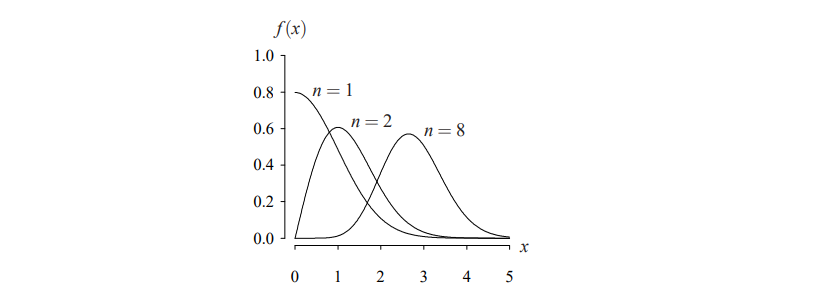
\includegraphics[width=1\textwidth]{image/卡方分布.png}
  \caption{卡方分布}
  \label{fig:example}
\end{figure}

 K 阶矩:

$$
\begin{aligned}
E(X^{k}) &= \int_0^{+\infty} x^{k} \cdot \dfrac{1}{2^{\frac{n}{2}}\Gamma(\dfrac{n}{2})}x^{^{\frac{n}{2}} - 1}e^{-\frac{x^{2}}{2}} \mathrm{d}x \\
\end{aligned}
$$

设 $\dfrac{x^{2}}{2}= t$,式子变为:
$$
\begin{aligned}
E(X^{k}) &= \dfrac{2^{\frac{k}{2}}}{\Gamma(\frac{n}{2})}\int_0^{+\infty} t^{\frac{n + k}{2} - 1}e^{-t}\mathrm{d}t \\
&= \dfrac{2^{k / 2}\Gamma(\frac{n + k}{2})}{\Gamma(n / 2)}
\end{aligned}
$$

 期望:

$$
E(X) = \dfrac{\sqrt{2}\Gamma(\frac{n + 1}{2})}{\Gamma(n / 2)}
$$

 方差:

$$
E(X^{2}) = \dfrac{2\Gamma(n / 2 + 1)}{\Gamma(n / 2)} = n
$$

所以

$$
D(X) = E(X^{2}) - E(X)^{2} = n^{2} - E(X)^{2}
$$

 性质:

1. 自由度:卡方分布的形状由自由度参数决定。自由度越高,分布越接近正态分布。

2. 相加性:如果$X1、X2、...、Xn$是n个独立的标准正态分布随机变量,那么它们的平方和$Σ(Xi^2)$服从自由度为n的卡方分布。

 应用:

1. 假设检验:卡方分布广泛用于假设检验,尤其是卡方检验。它用于比较观测值与期望值之间的差异,以评估统计显著性,例如在拟合度检验、独立性检验和同质性检验中的应用。

2. 方差分析:在方差分析中,卡方分布用于计算F统计量的分布,以检验不同组之间的均值是否具有显著差异。

3. 生物统计学:在生物学和医学研究中,卡方分布用于分析分布数据、遗传分析、药效学试验和流行病学研究等。

4. 数据转换:卡方分布经常用于对数据进行正态化或变换,以满足正态性假设,从而在统计建模中更好地应用线性模型。

5. 质量控制:在质量控制和制造过程中,卡方分布用于分析过程数据、检测不良品率、评估产品质量和生产能力。

\section{狄拉克分布(Dirac Distribution)}


狄拉克分布也称为狄拉克δ函数,是一种不连续的概率分布,通常在数学和物理学中用于描述点态分布的情况。

 性质:

1. 点态分布:狄拉克分布是一种点态分布,它的概率密度函数在一个单一的点上有非零值,而在其他点上为零。这个点通常用δ符号表示,例如δ(x - a),其中a是分布的点位。

2. 单位面积:狄拉克分布满足积分为1的条件,即$∫δ(x - a) dx = 1$,这意味着整个概率质量集中在点a上。

3. 无限高度:狄拉克分布在点a处的概率密度函数值为正无穷,即δ(a) = ∞。

 应用:

1. 量子力学:在量子力学中,狄拉克分布用于描述粒子的位置和动量。位置和动量算符的期望值通常用狄拉克分布表示。

2. 信号处理:狄拉克δ函数经常用于信号处理中,特别是在连续时间信号和离散时间信号的分析中,以描述脉冲信号或离散事件的发生。

3. 物理学:在物理学中,狄拉克分布用于建模点电荷分布或理想化的物体,如质点或无限薄的物体。

4. 数学分析:在数学中,狄拉克δ函数是分布理论的基础,用于表示广义函数和广义导数。它在微积分、偏微分方程和泛函分析中有应用。

\section{迪利克雷分布(Dirichlet Distribution)}

 迪利克雷过程(Dirichlet Process, DP)

迪利克雷分布是一种「分布的分布」,有两个参数 $\alpha, G_0$ 确定,即 $G \sim DP(\alpha, G_0)$,$\alpha$ 是分布参数,它的值越大,分布越接近于基分布,其值越小,分布越 Concentrated,$G_0$ 是基分布。

 什么时候需要迪利克雷分布?

我们有一组来源于混合高斯分布的数据集,希望对其进行聚类,然而我们并不知道这组数据是由几组高斯分布生成的。

\begin{figure}[H]
  \centering
  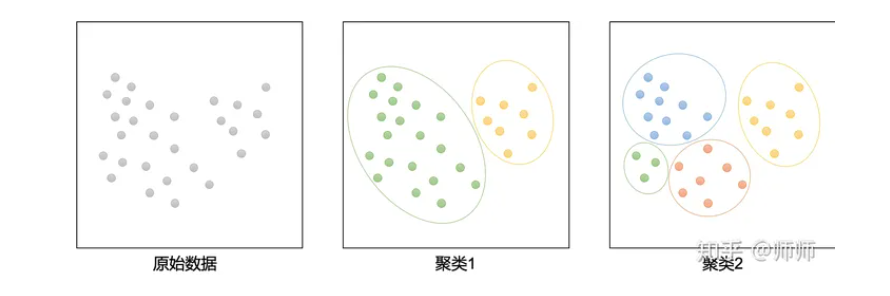
\includegraphics[width=1\textwidth]{image/狄利克雷过程.png}
  \caption{狄利克雷过程}
  \label{fig:example}
\end{figure}

 概率密度函数:

维度 $k \geq 2$ 的狄利克雷分布在参数 $\alpha_1, \alpha_2, ..., \alpha_k > 0$ 上,基于欧几里得空间 $\R^{k - 1}$ 里的勒贝格测度有个概率密度函数:

$$
f(x) = \dfrac{1}{\text{B}(\alpha)} \prod\limits_{i = 1}^{K}x_i^{\alpha_i - 1}
$$

其中,$\sum\limits_{i = 1}^{K} x_i = 1$

 期望:

$$
E(X_i) = \dfrac{\alpha_i}{\sum_k\alpha_k}
$$

 性质:

1. 多维分布:迪利克雷分布通常用于表示多维随机变量的联合分布,这些随机变量通常表示多个类别或选项的概率分布。它是多项分布的共轭先验,用于贝叶斯推断。

2. 参数:迪利克雷分布有一个参数向量α,该向量决定了分布的性质。参数α的每个分量表示对应类别的先验估计,它们通常是正数。

3. 概率密度函数:迪利克雷分布的概率密度函数是复杂的,通常表示为Dir(x|α)。它用于计算多维随机变量的联合概率密度。

4. 均值和方差:迪利克雷分布的均值是由参数α决定的,方差也与参数α有关。

 应用:

1. 主题建模:在自然语言处理中,迪利克雷分布常用于主题建模,如Latent Dirichlet Allocation(LDA)模型。LDA用于分析文本数据,将文档表示为多个主题的混合,每个主题由单词分布表示。

2. 多项分布的先验:迪利克雷分布是多项分布的共轭先验,因此它在统计推断中常用于估计多项分布的参数。这在分类、文档建模和图像分析中很有用。

3. 概率分布建模:迪利克雷分布可用于建模多个随机变量的联合分布,例如多类别文档的标签分布、多项选择的分布概率等。

4. 贝叶斯推断:迪利克雷分布在贝叶斯统计中具有重要作用,它用于估计参数的后验分布,结合观测数据进行推断。

\section{帕累托分布(布拉德福分布, Pareto Distribution)}
这个分布是是从大量真实世界的现象中发现的[幂定律](https://zh.wikipedia.org/wiki/冪定律)分布。这个分布在经济学以外,也被称为布拉德福分布。

 分布函数:

$$
P(X > x) = \left(\dfrac{x}{x_{\min}} \right)^{-k}
$$

其中,x 是任何一个大于 $x_{\min}$ 的数,$x_{\min}$ 是 X 最小的可能值(正数)。

 概率密度:

$$
\begin{aligned}
p(x) = \begin{cases}
0 \quad x < x_{\min} \\
\\
\\
\dfrac{kx_{\min}^{k}}{x^{k + 1}} \quad x > x_{\min}

\end{cases}
\end{aligned}
$$



帕累托分布属于连续概率分布。「齐夫定律」也被称为「Zeta 分布」,也可以被认为是在离散概率分布中的帕累托分布。

\begin{figure}[H]
  \centering
  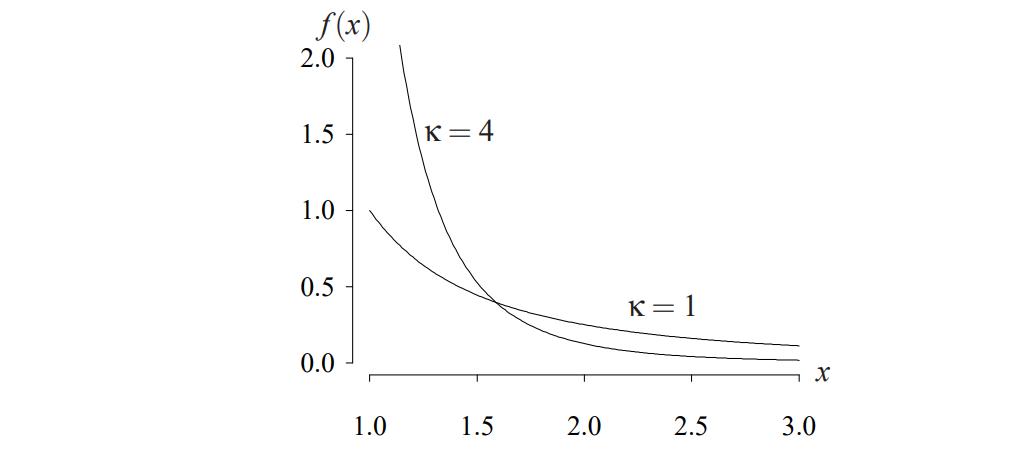
\includegraphics[width=1\textwidth]{image/帕累托分布.png}
  \caption{帕累托分布}
  \label{fig:example}
\end{figure}

 期望:

$$
E(X) = \int_0^{+\infty} x\cdot f(x) \mathrm{d}x = \dfrac{x_\min k}{k - 1}
$$

 方差:

$$
D(X) = \dfrac{x_\min}{k - 1}\sqrt{\dfrac{k}{k - 2}}
$$

 应用:

1. 财富在个人之间的分布

2. 人类居住区的大小

3. 对维基百科条目的访问

4. 接近绝对零度时,玻色一爱因斯坦疑聚的团簇

5. 在互联网流量中文件尺寸的分布

6. 油田的石油储备数量

7. 龙卷风带来的灾难的数量

 引申:

帕累托法则(Pareto Principle),或者叫做「二八定律」,「关键少数法则」,「巴莱多定律」。这个定律指出,约仅有 20% 的因素影响了 80% 的结果。也就是说,所有变因中,最重要的仅有 20%,虽然剩余的 80% 占了大多数。


\section{反正弦分布(Arcsin Distribution)}


 符号:$X \sim \text{arcsin}(x)$

 概率密度函数:

$$
f(x) = \dfrac{1}{\pi \sqrt{x(1 - x)}} \quad 0 < x < 1
$$

\begin{figure}[H]
  \centering
  
\includegraphics[width=1\textwidth]{image/反正弦分布.png}
  \caption{反正弦分布}
  \label{fig:example}
\end{figure}

 累计分布函数:

$$
F(x) = P(X \leq x) = \dfrac{\pi + 2\arcsin(2x - 1)}{2\pi}
$$

 期望:

$$
E(X) = \dfrac{1}{2}
$$

 方差:

$$
D(X) = \dfrac{1}{8}
$$

 性质:

对于积分 $\int_{a}^{b}\dfrac{\mathrm{d}x}{\sqrt{(x - a)(b - x)}}$ 它的结果是$\pi$

对于这样类型的积分,我们一般是通过换元进行计算 $x  =a\cos^{2}\theta + b\sin^{2}\theta$,那么原来的积分可以变为一个简单的积分:

$$
\int_a^{b}\dfrac{\mathrm{d}x}{\sqrt{(x - a)(b - x)}} = 2\int_0^{\frac{\pi}{2}} \mathrm{d}\theta = \pi
$$

对于这个式子的含义继续深究

\begin{figure}[H]
  \centering
  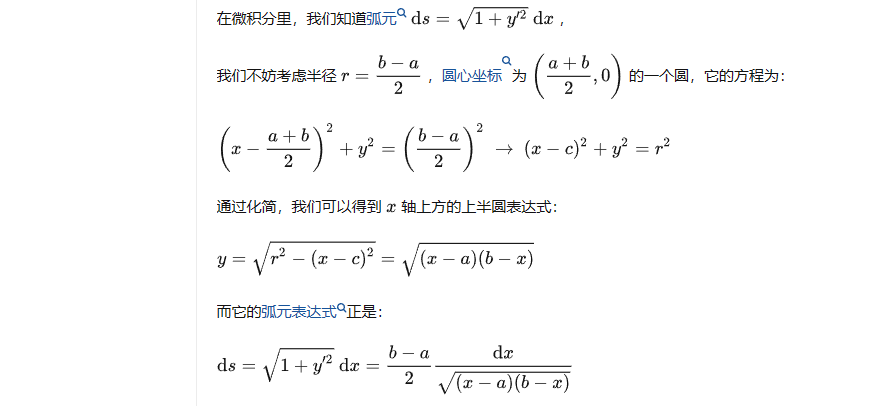
\includegraphics[width=1\textwidth]{image/反正弦分布1.png}
  \label{fig:example}
\end{figure}

所以原来的定积分就正好代表了上半圆的弧长,也就是整个圆的半周长。

\begin{figure}[H]
  \centering
  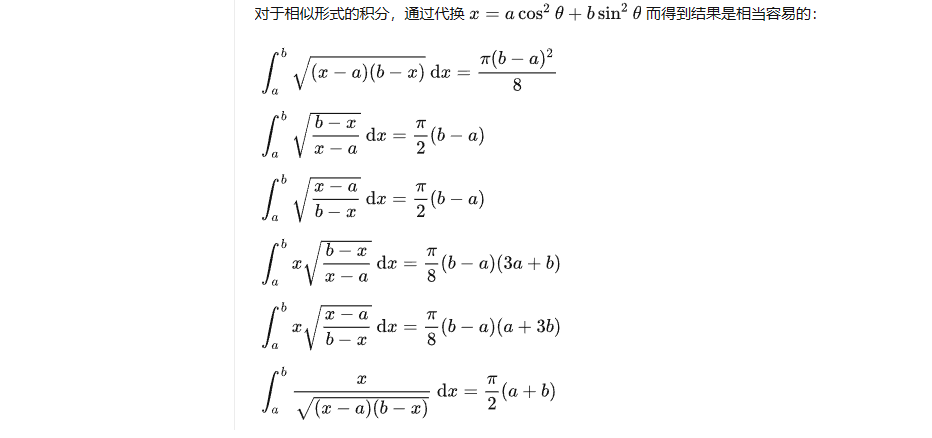
\includegraphics[width=1\textwidth]{image/反正弦分布2.png}
  \label{fig:example}
\end{figure}

\chapter{特征函数}

特征函数是概率论中非常重要的工具,它有点像分析里面的Fourier变换。特征函数可以用于求实值随机变量的期望和方差;同时也可用于求某个随机变量的分布律,这是因为,特征函数有一个最重要的结果,就是特征函数唯一确定一个分布律。

\section{特征函数}

设 $\mu$ 是 $\mathbb{R} ^{m}$ 上的概率测度,定义:

$$
\mu(\theta) = \int_{\mathbb{R} ^{m}} e^{i<\theta, x>} \mu \mathrm{d}x = E(e^{i<\theta, x>}), \theta \in \mathbb{R}^{m}
$$

为 $\mu$ 的特征函数,其中 $<\cdot, \cdot>$ 表示内积。

(1) 若 $X \in L^{1}$,则 $\mu$ 的一阶倒数存在,并且:

$$
\dfrac{\partial \mu}{\partial \theta_{j}}(\theta) = i \int_{\mathbb{R}^{m}} x_j e^{i<\theta, x>} \mu \mathrm{d}x
$$

特别的,
$$
\dfrac{\partial \mu}{\partial \theta_{j}}(0) = i \int_{\mathbb{R}^{m}} x_j \mu \mathrm{d}x = iE(X_j)
$$

因此 $\nabla\mu(0) = iE(X)$。

(2) 若 $X \in L^{2}$,则 $\mu$ 的二阶倒数存在,并且:

$$
\dfrac{\partial^{2}\mu}{\partial \theta_k \partial \theta_j}(\theta) = -\int_{\mathbb{R}^{m}} x_k x_j  e^{i<\theta, x>} \mu \mathrm{d} x
$$

特别地,

$$
\dfrac{\partial^{2}\mu}{\partial \theta_k \partial \theta_j}(0) = -\int_{\mathbb{R}^{m}} x_k x_j \mu \mathrm{d} x
$$

如果 $m = 1$,那么就有 $\mu^{''}(0) = -E(X^{2})$。如果 $m = 2$ 并且 $X$ 是零均值的,则 $\mu$ 的 Hesse 矩阵在 0 处的值,等于 -Cov(X)。

\section{正态分布特征函数}
\begin{align*}
\varphi(t) &= E(e^{itx}) \\ &= \dfrac{1}{\sqrt{2\pi} \sigma} \int_{-\infty}^{+\infty} e^{itx} e^{-\frac{(x-\mu)^{2}}{2\sigma^{2}}} \mathrm{d}x \\
&= \dfrac{1}{\sqrt{2\pi} \sigma}\int_{-\infty}^{+\infty} e^{-(\frac{(x-\mu)^{2}}{2\sigma^{2}} - itx)} \mathrm{d}x \\ 
\text{令} \dfrac{x- \mu}{\sigma} = m \\
&= \dfrac{1}{\sqrt{2\pi}\sigma}\int_{-\infty}^{+\infty}e^{-(\frac{m^{2}}{2} - it\sigma m - it\mu)} \mathrm{d}m \\
&= \dfrac{1}{\sqrt{2\pi}}e^{it\mu}e^{\frac{(it\sigma)^{2}}{2}} \int_{-\infty}^{+\infty}e^{-\frac{1}{2}(m - it\sigma)^{2}} \mathrm{d}x \\
&= \dfrac{1}{\sqrt{2\pi}} e^{it\mu} e^{\frac{(it\sigma)^{2}}{2}} \sqrt{2\pi} \\
 &= e^{it\mu} e^{\frac{(it\mu)^{2}}{2}}  \\
 &= e^{it\mu-\frac{1}{2}\sigma^{2}t^{2}}
\end{align*}

所以,

\begin{align*}
    E(X) &= \dfrac{\nabala \varphi(0)}{i} = \mu \\D(X) &= -\varphi^{''}(0) - E(X^{2}) = \mu^{2} + \sigma^{2} - \mu^{2} = \sigma^{2}
\end{align*}


\section{均匀分布特征函数}
\begin{align*}
    \varphi(t) &= E(e^{itx}) \\
    &= \int_a^{b} \dfrac{e^{itx}}{b - a} \mathrm{d}x \\
    &= \dfrac{e^{itb} - e^{ita}}{it(b - a)}
\end{align*}

所以,

\begin{align*}
    E(X) &= \dfrac{\varphi^{'}(0)}{i} = \dfrac{a + b}{2}\\
    D(X) &= E(X^{2}) - E(X)^{2} = -\mu^{''}(0) - E(X)^{2} = \dfrac{(b-a)^{{2}}}{12}
\end{align*}
\section{指数分布特征函数}
\begin{align*}
\varphi(t) &= E(e^{itx}) \\
&= \int_0^{+\infty} e^{itx} \lambda e^{-\lambda x}\mathrm d{x} \\
&= \lambda \int_0^{+\infty} e^{-(\lambda - it)} \mathrm{d}x \\
&= \lambda(-\dfrac{1}{\lambda - it}e^{(\lambda - it)x} |_0^{+\infty}) \\
&= \lambda \dfrac{1}{\lambda - it} \\
&= \left( \dfrac{\lambda - it}{\lambda}\right)^{-1} \\
&= (1 - \frac{it}{\lambda})^{-1}
\end{align*}

所以,

\begin{align*}
E(X) &= \dfrac{\varphi^{'}(0) }{i} = \dfrac{\frac{1}{\lambda}\cdot i }{i}  =\frac{1}{\lambda} \\
D(X) &= E(X^{2}) - E(X)^{2} \\
&= -\varphi(0)^{''} - E(X)^{2} \\
&= \dfrac{1}{\lambda^{2}}
\end{align*}

\section{伽马分布特征函数}
\begin{align*}
\varphi(t) &= \int_0^{+\infty} \dfrac{\lambda^{\alpha}}{\Gamma(\alpha)} \dfrac{x^{\alpha - 1}}{e^{\lambda x}} e^{itx} \mathrm{d} x \\
&= (1 - \dfrac{it}{\lambda})^{-\alpha}
\end{align*}

所以,

\begin{align*}
    E(X) &= \dfrac{\varphi^{'}(0) }{i} = \dfrac{\alpha}{\lambda}\\
    D(X) &= E(X^{2}) - E(X)^{2} = \dfrac{\alpha(\alpha + 1)}{\lambda}
\end{align*}

\section{贝塔分布特征函数}
贝塔函数的特征函数推导复杂,也不常用,略。

\section{卡方分布特征函数}
卡方分布是伽马函数的特例,$\chi^{2}(n) = \Gamma(\frac{n}{2}, \frac{1}{2})$

所以,

\begin{align*}
    \varphi(t) = (1 - 2it)^{-\frac{n}{2}}
\end{align*}

\section{泊松分布特征函数}
\begin{align*}
    \varphi(t) &= E(e^{itx}) \\
    &= \sum\limits_{x = 0}^{+\infty} e^{itx} \cdot e^{-\lambda \dfrac{\lambda^{x}}{x!}} \\
    &= e^{-\lambda} \sum\limits_{x = 0}^{+\infty}\dfrac{(e^{it} \cdot \lambda)^{x}}{x!} \\
    &= e^{\lamda(e^{it} - 1)} 
\end{align*}

所以,
\begin{align*}
    E(X) &= \varphi^{'}(0) / i = \lambda\\
    D(X) &= E(X^{2}) - E(X)^{2} = \lambda
\end{align*}

\end{document}